\chapter{User documentation}
\label{ch:user}

\section{General Requisite}

The application is for the internal usage within SAP for the parcel collection service providing to the employees. The solution consists of 6 applications as tiles on the Fiori launchpad: \textbf{My packages}, \textbf{Pickup packages}, \textbf{Register Packages}, \textbf{Manage packages}, \textbf{Manage Companies} and \textbf{Manage Storages} partitioned into 3 sections: \textbf{My Home}, \textbf{Pacel Handling}, \textbf{Administration}, as shown in the diagram.

\begin{figure}[H]
	\centering
	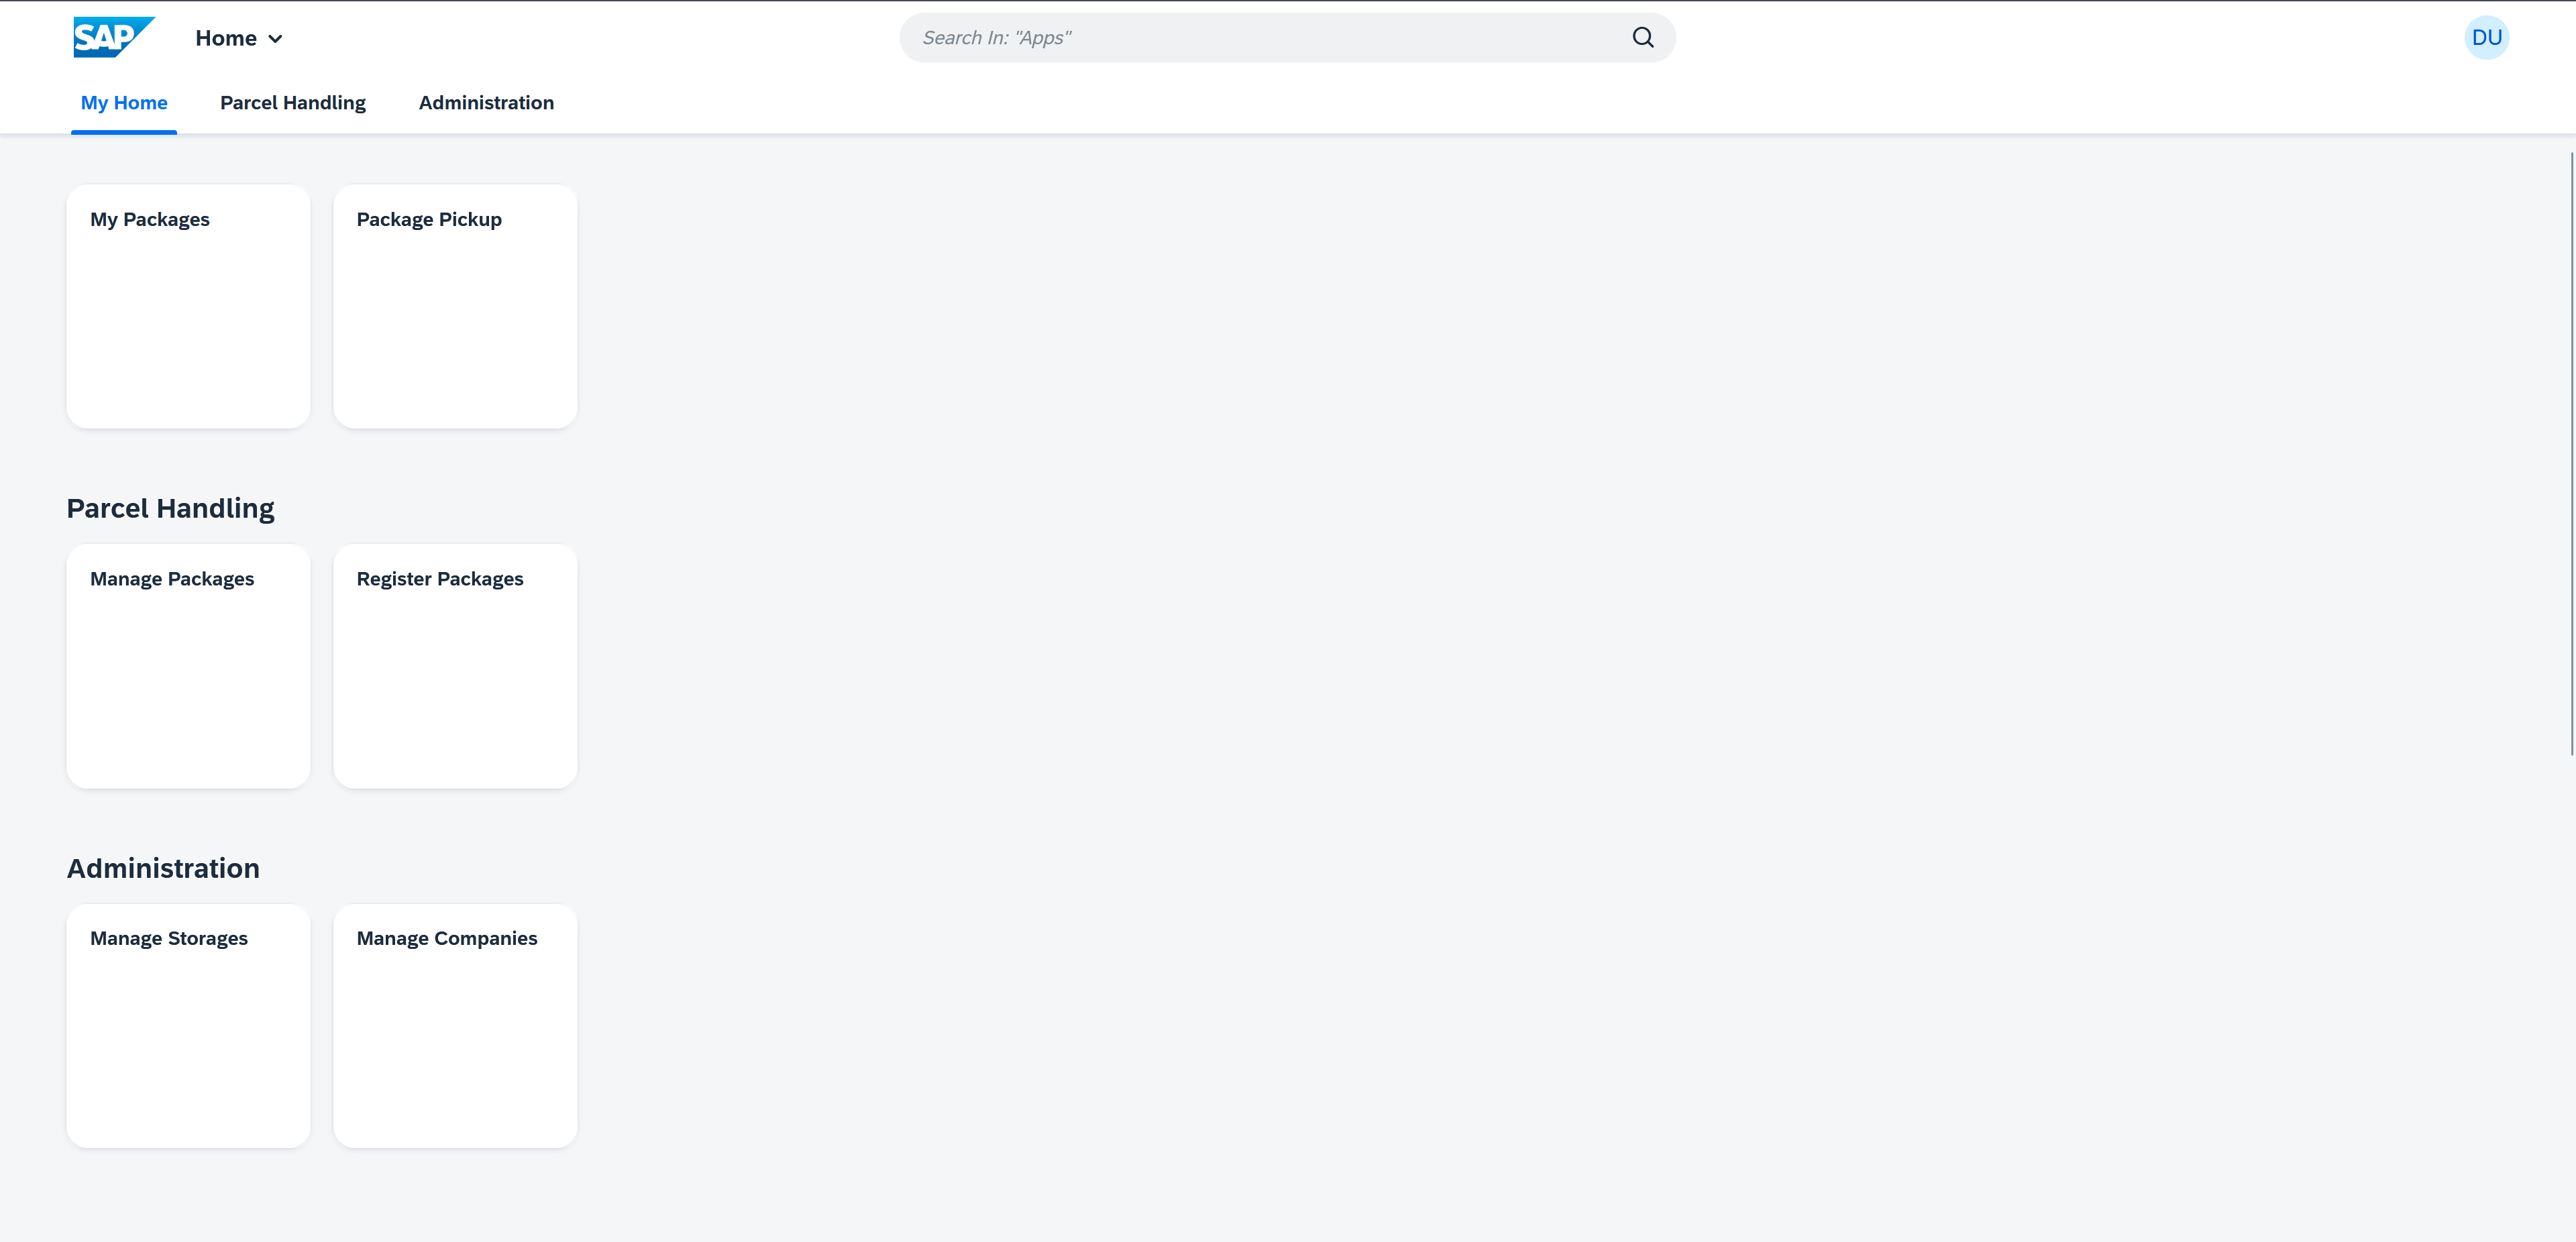
\includegraphics[width=1\linewidth]{images/user_doc/overviews/sandbox.png}
	\caption{Application Launch Screen}
	\label{fig:ApplicationLaunchScreen}
\end{figure}


In order to use any of the application, one has to hold an SAP registered device (computer/tablet/phone) and is able to use a supported browser with stable internet connection. In order to use \textbf{Pickup packages} application, one has to hold an SAP registered smart phone. 

In order to mock use the application in local environment, please move the the developer chapter. 

Four different roles are specified for the application and one is limited to dedicated usage of the applications, depends on the role. In the coming sections the usage guides are documented partitioned by the roles. Hereby lists the meaning of each role under the thesis context:

\begin{description}
	\item[End User] any SAP employee who holds an SAP registered device and would like to use the parcel collection service.
	\item[Receptionist] Registered receptionist (in database) working at the reception and is responsible to serve the parcel collection service.
	\item[Facility Manager] Authorised user who is responsible for maintaining the delivery companies and storage slots information.
	\item[Administrator] The master user who can access to any of the applications.
\end{description}

In case one is accessing the applications through browser from BTP platform, the login process is done automatically. Otherwise, if one is running the application locally, a browser pop up will appear and mock user should be entered. The different mock user login info can be find in the developer documentation security chapter.

\begin{figure}[H]
	\centering
	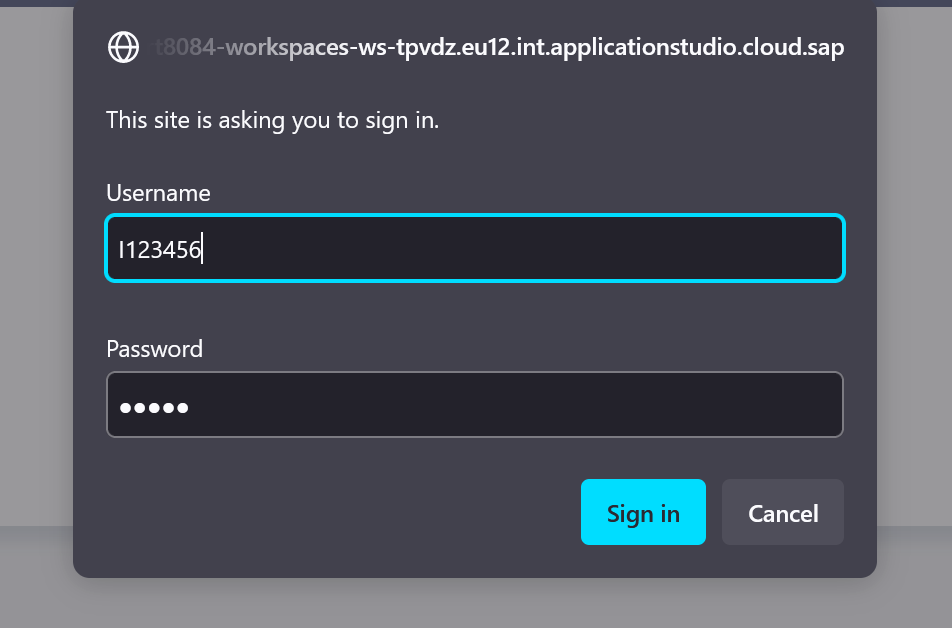
\includegraphics[height=200pt]{images/user_doc/overviews/localLogin.png}
	\caption{Local Login Pop Up}
	\label{fig:LocalLoginPopUp}
\end{figure}

In the case of any user trying to accessing an unauthorised application, connection will fail.

\begin{figure}[H]
	\centering
	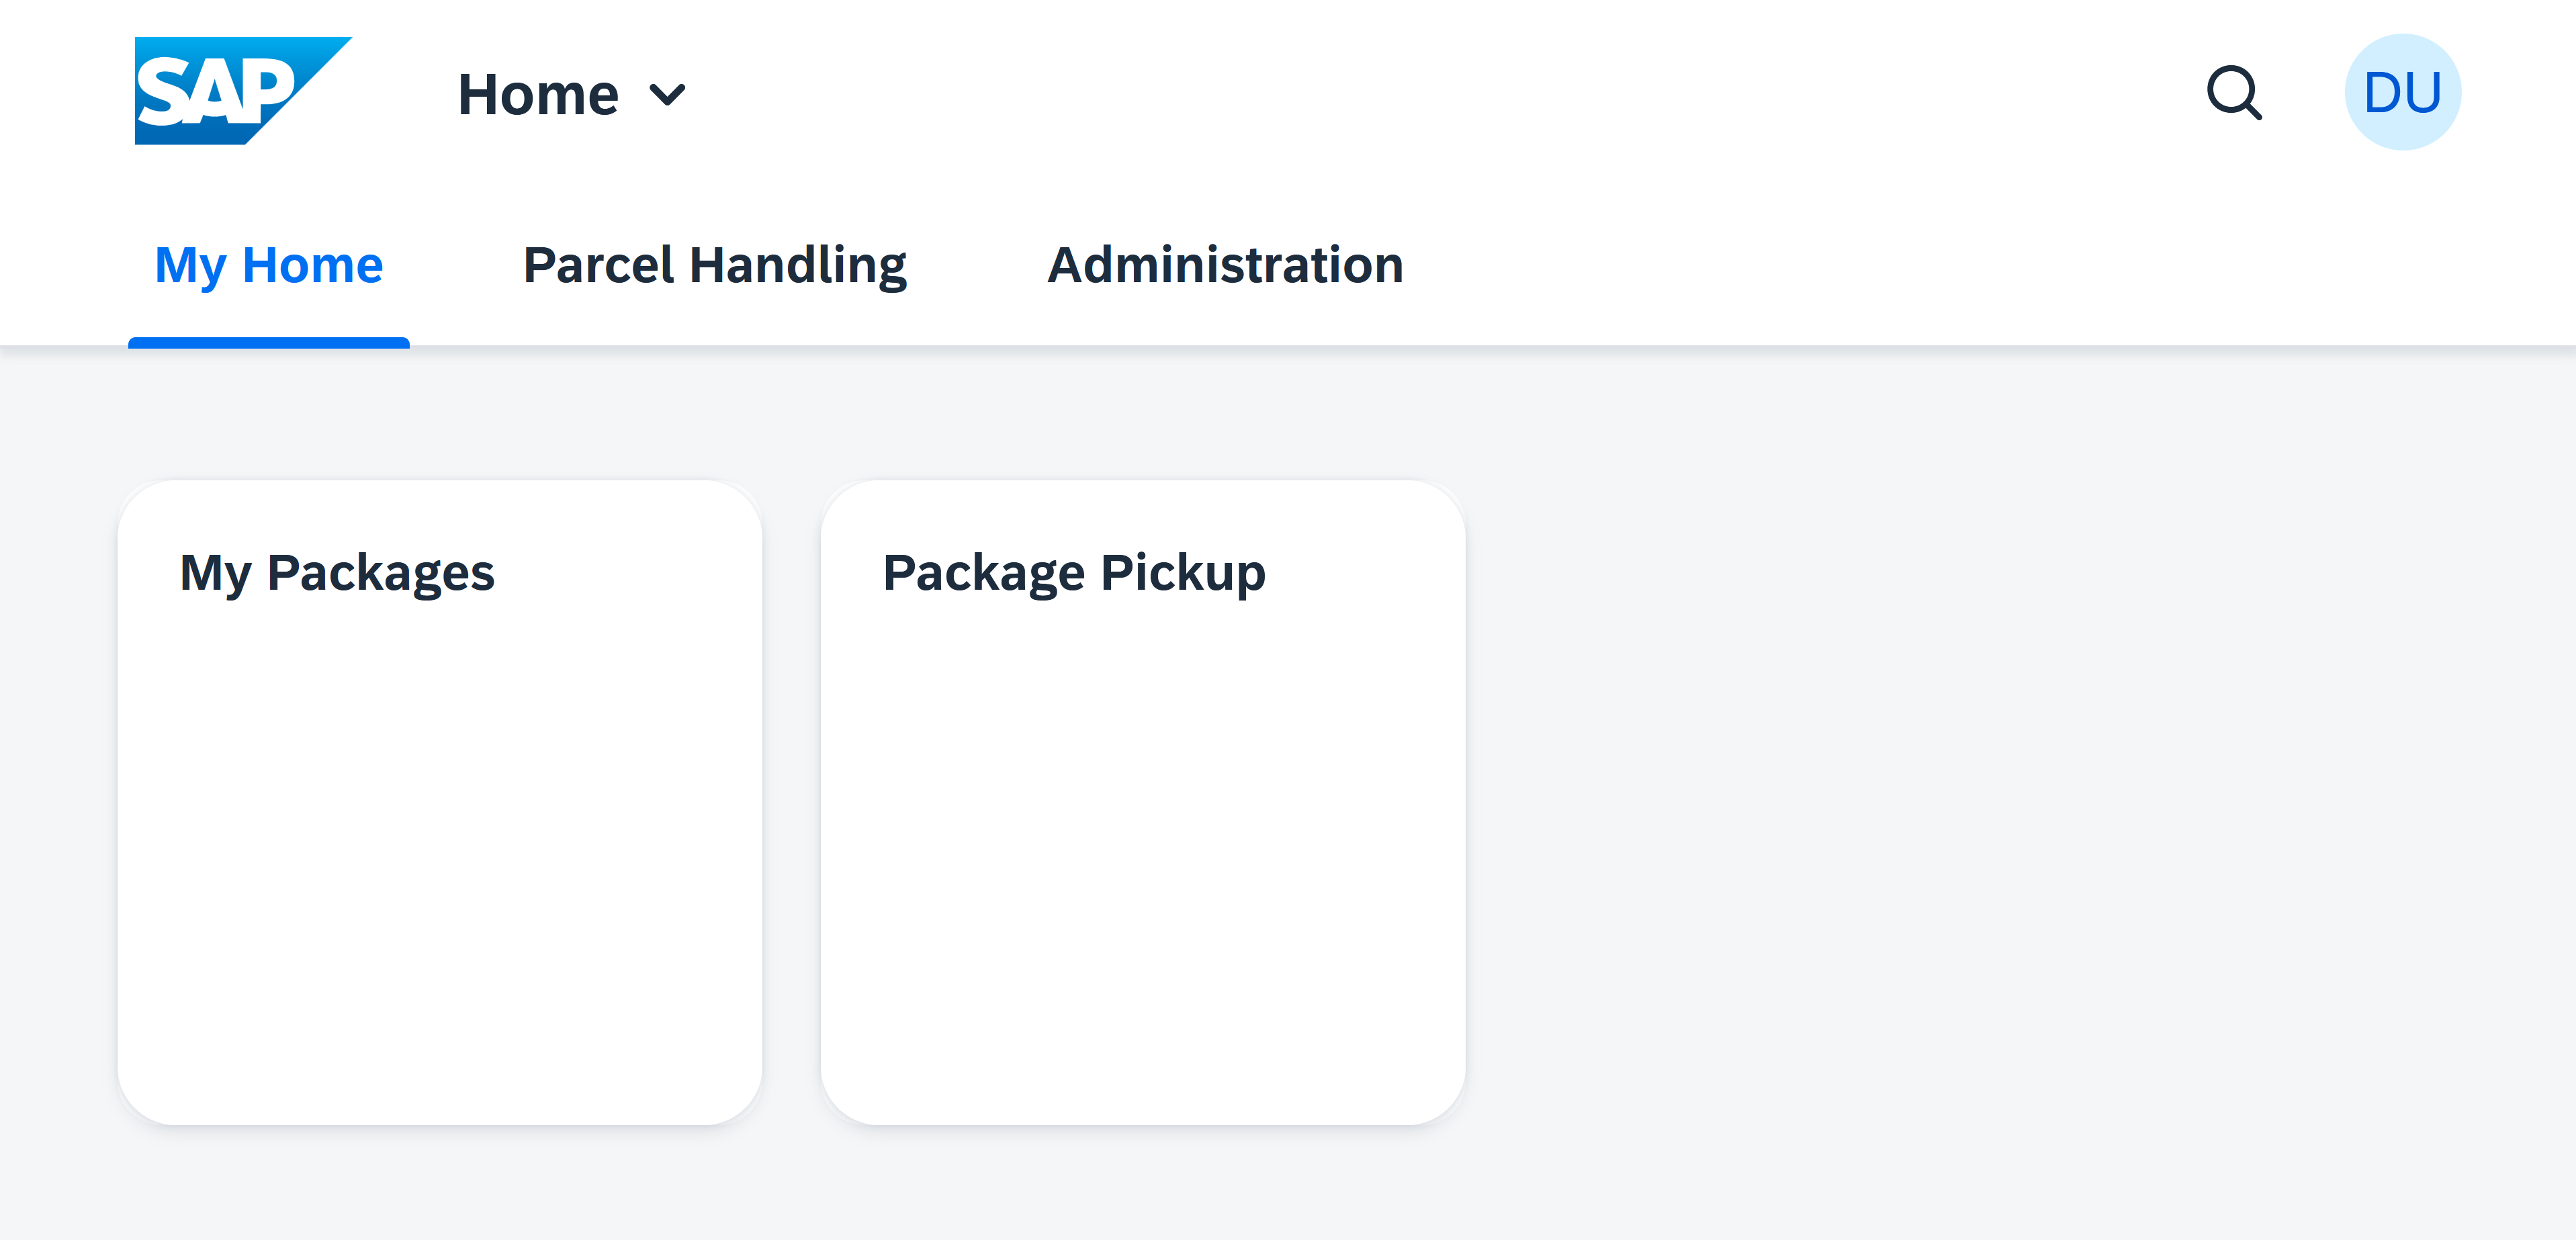
\includegraphics[width=1\linewidth]{images/user_doc/overviews/MyHomeTab.png}
	\caption{Illegal Access to Unauthorised Applications}
	\label{fig:IllegalAccesstoUnauthorised Applications}
\end{figure}

\pagebreak

\section{End User}

As a logged in \textbf{End User}, one is granted to access the two applications under the \textbf{My Home} section, namely \textbf{My Packages} and \textbf{Package Pickup}. One can quick jump to the section by left clicking the "My Home" tab. One can enter the application by left click the tiles.

\begin{figure}[H]
	\centering
	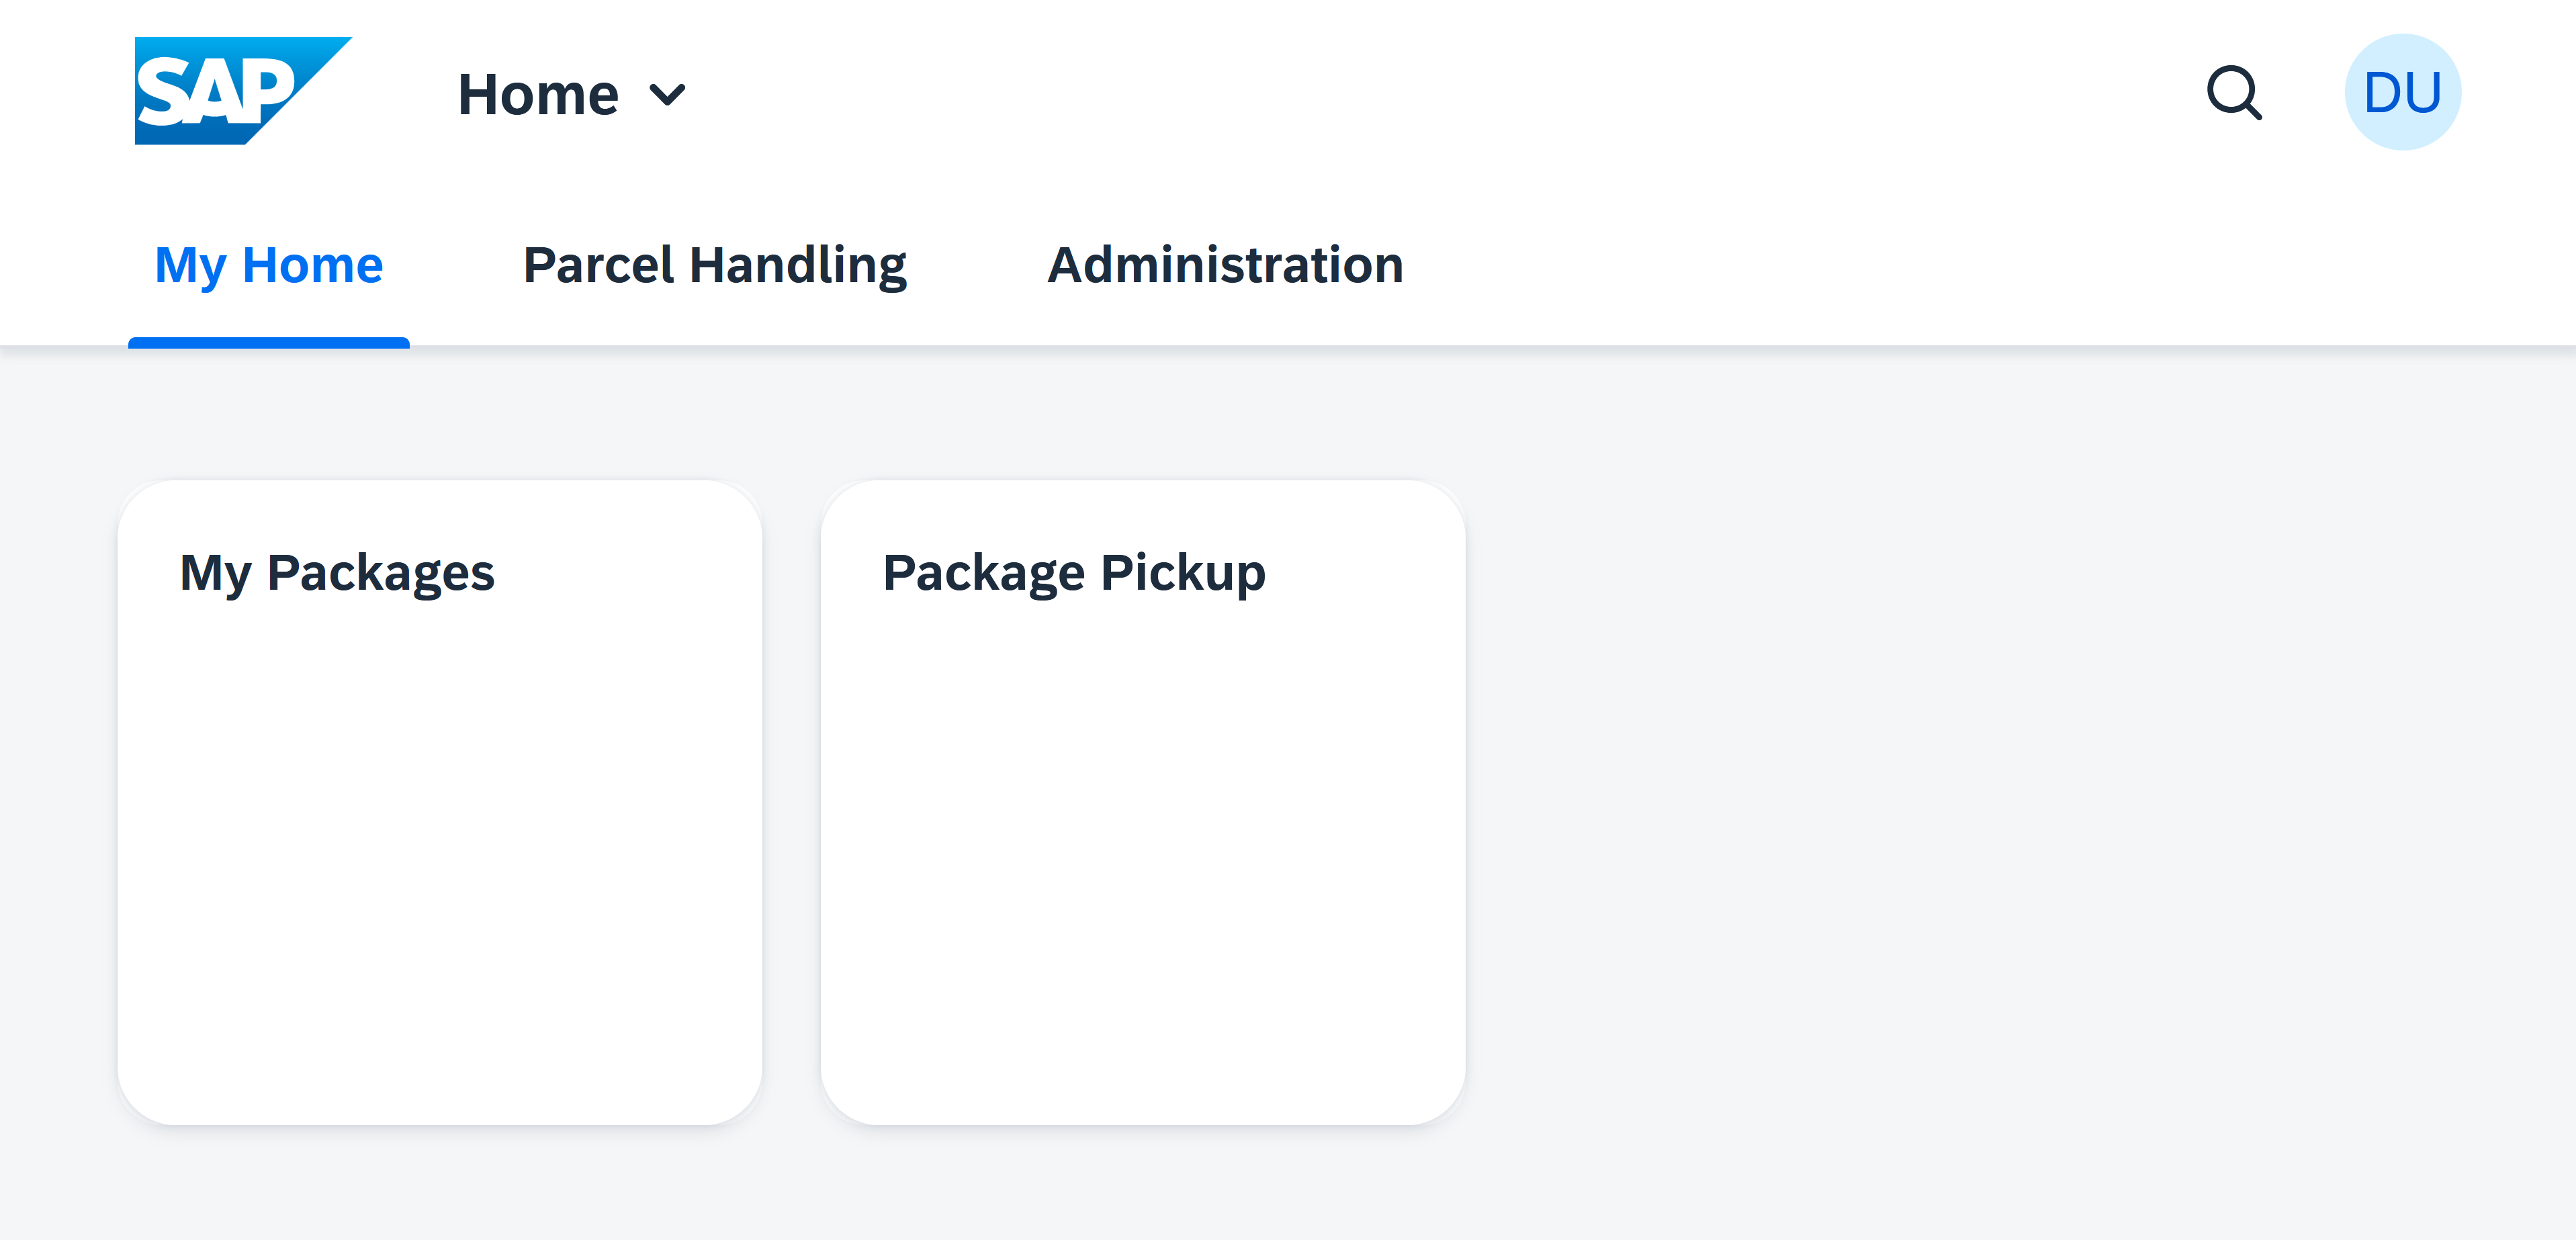
\includegraphics[width=1\linewidth]{images/user_doc/overviews/MyHomeTab.png}
	\caption{End User Applications}
	\label{fig:EndUserApplications}
\end{figure}



\subsection{My Packages}

\subsection{Package Pickup}
The \textbf{Package Pickup} application is used to pick up any confirmed parcels (registered at the reception and confirmed with a storage slot) of the logged in user. One can only see one's own confirmed packages. 

Warning: The application supports only from mobile devices. In case an employee is unable to access his or her mobile at the moment of pickup, he or she shall ask the receptionist to pickup the package for him or her.

\bigskip

\subsubsection{Home Screen - Selection}
As an \textbf{End User}, after clicking at the application tile, is redirected to the "Home Screen". If there exists at least one package to pickup, the home screen shows the list of packages. The list items lists \textbf{the type with icon, the delivery company, the registration time and the location} of the packages. If no package exists to pickup, it shows only the no package info. The package list title shows the total number of packages that can be pickup.

In case there are existing packages, one can select one or multiple packages from the list to pickup. 

In case there are existing packages, one can tick/untick the "Toggle All" selection box to select or deselect the package all at once. 

\begin{figure}[H]
	\centering
	\subcaptionbox{Home Screen with Packages}{
		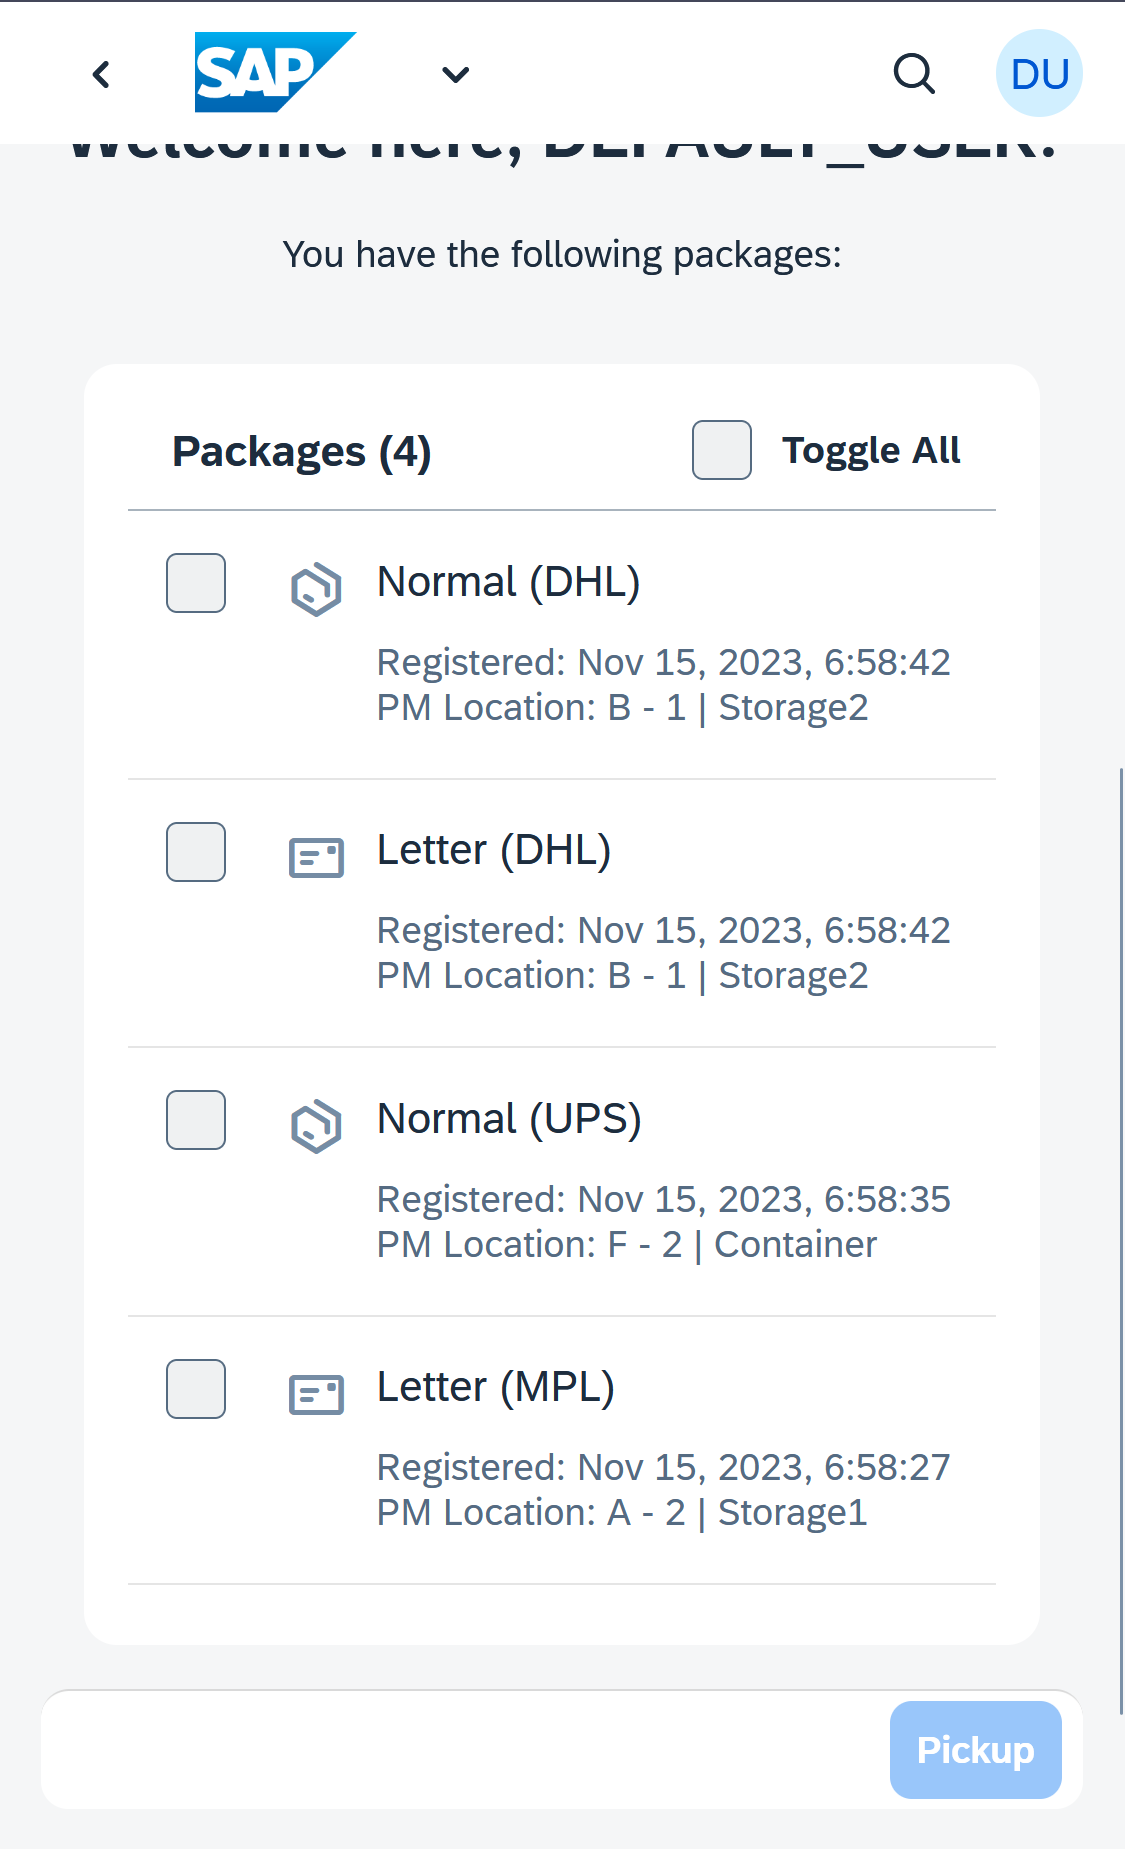
\includegraphics[width=0.45\linewidth]{images/user_doc/pickup/HomeScreenList.png}}
	\hspace{5pt}
	\subcaptionbox{Home Screen without Packages}{
		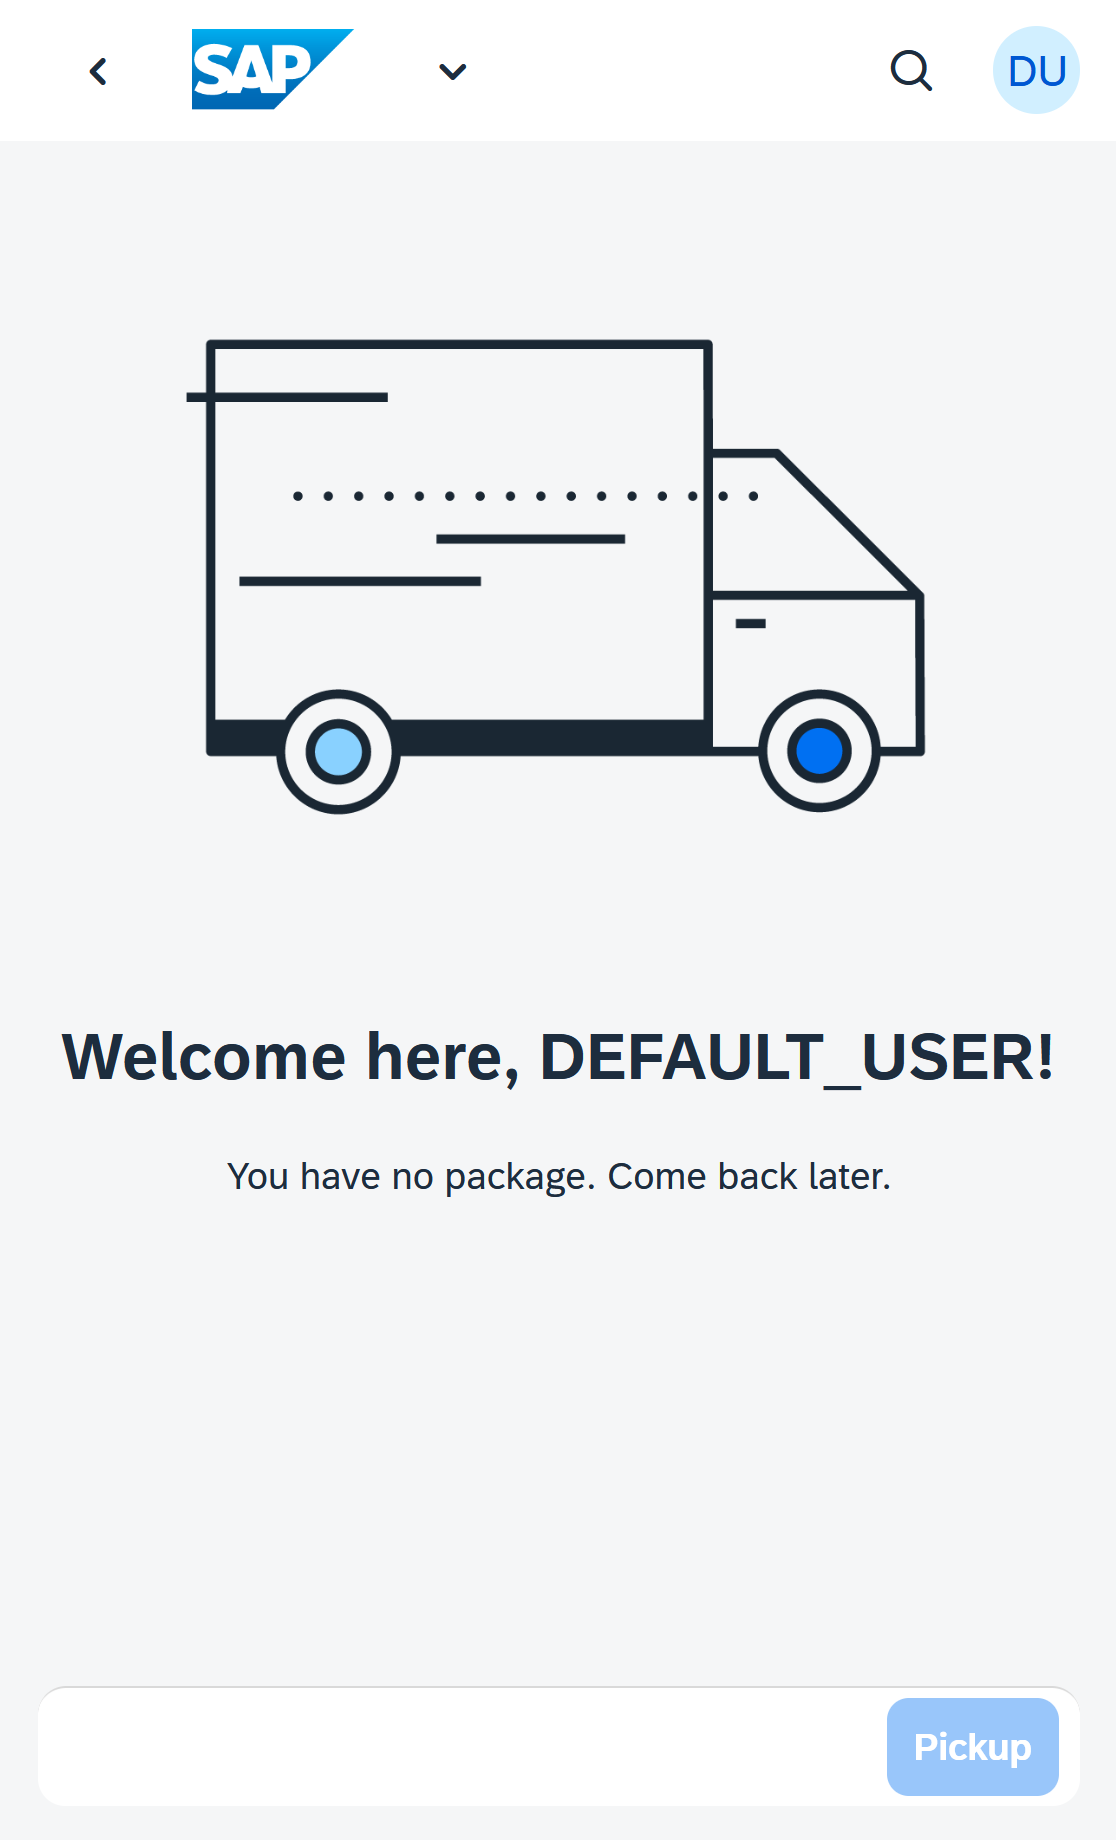
\includegraphics[width=0.45\linewidth]{images/user_doc/pickup/HomeScreenNoPackage.png}}
	\caption{Pickup Home Screen - Package Existence Guide}
	\label{fig:PickupHomeScreen-1}
\end{figure}

\begin{figure}[H]
	\centering
	\subcaptionbox{Home Screen Single Selection}{
		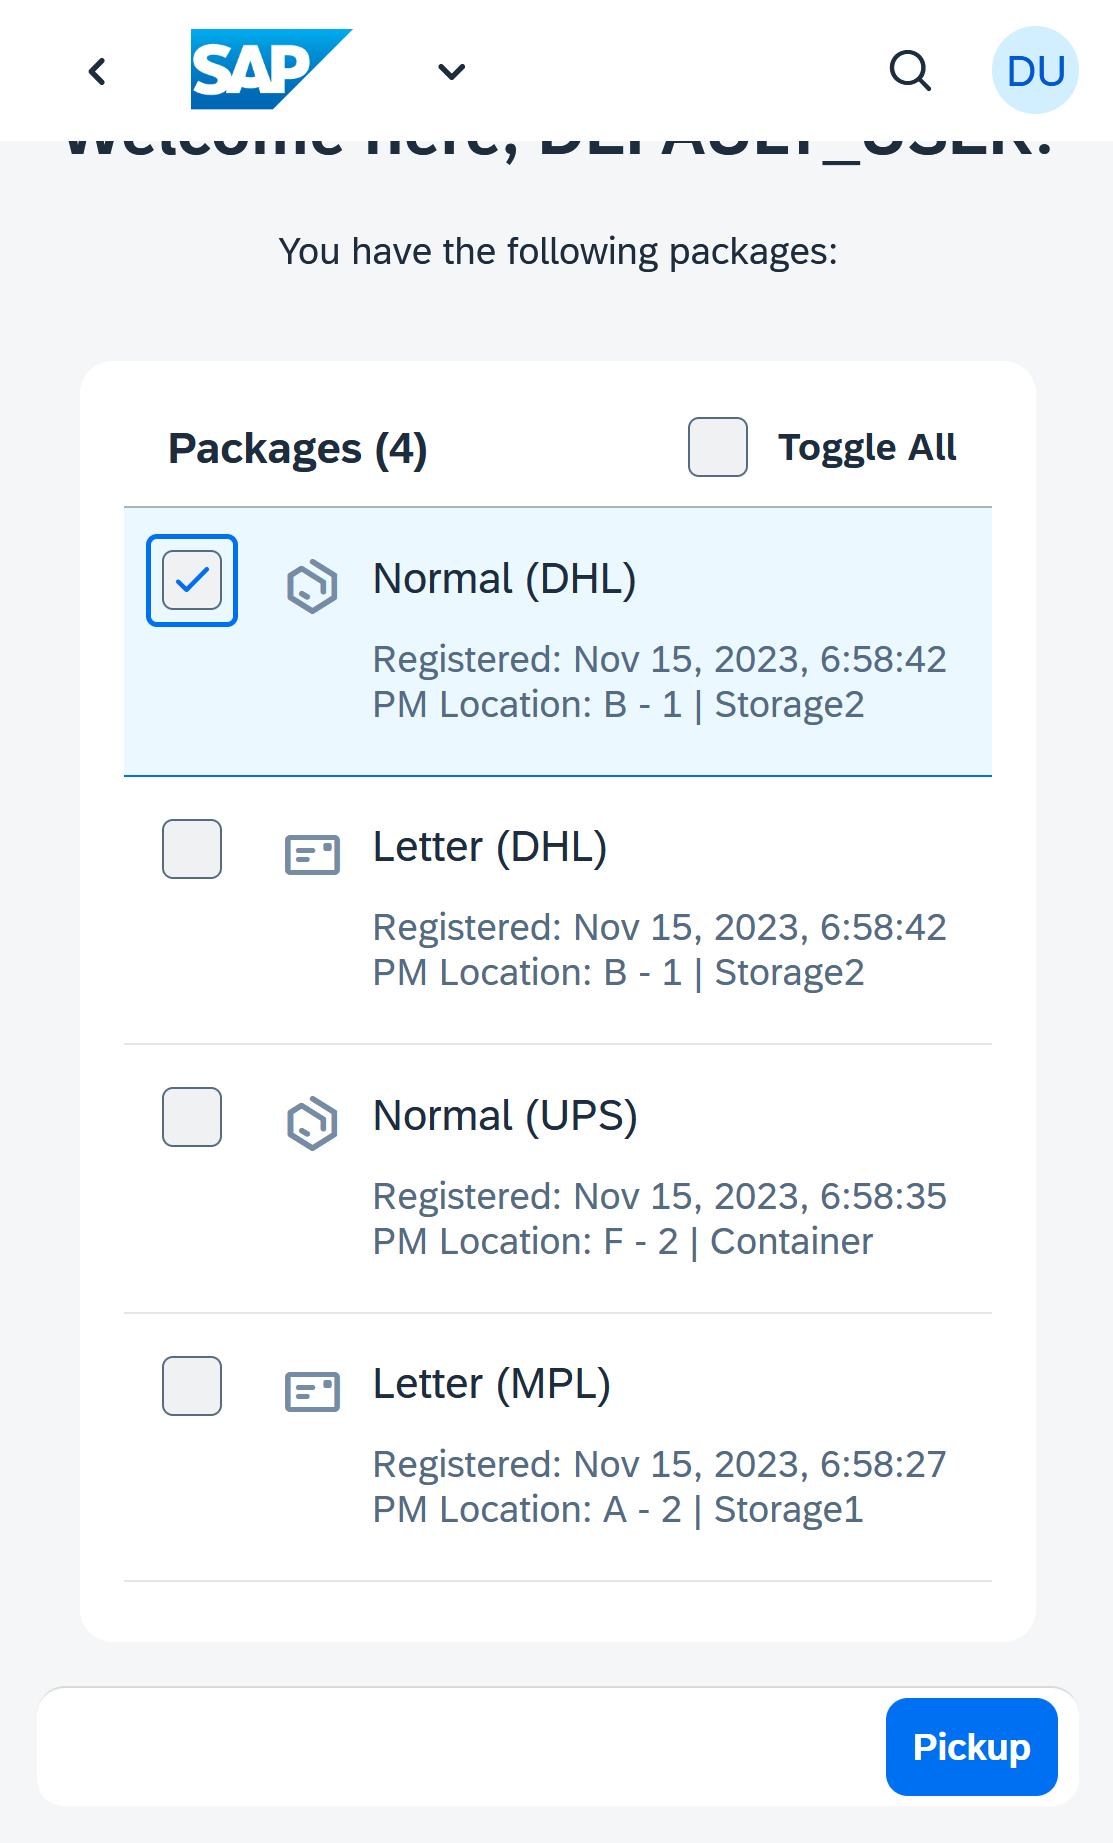
\includegraphics[height=260pt]{images/user_doc/pickup/HomeScreenSelectOne.png}}
	\hspace{5pt}
	\subcaptionbox{Home Screen Multiple Selection}{
		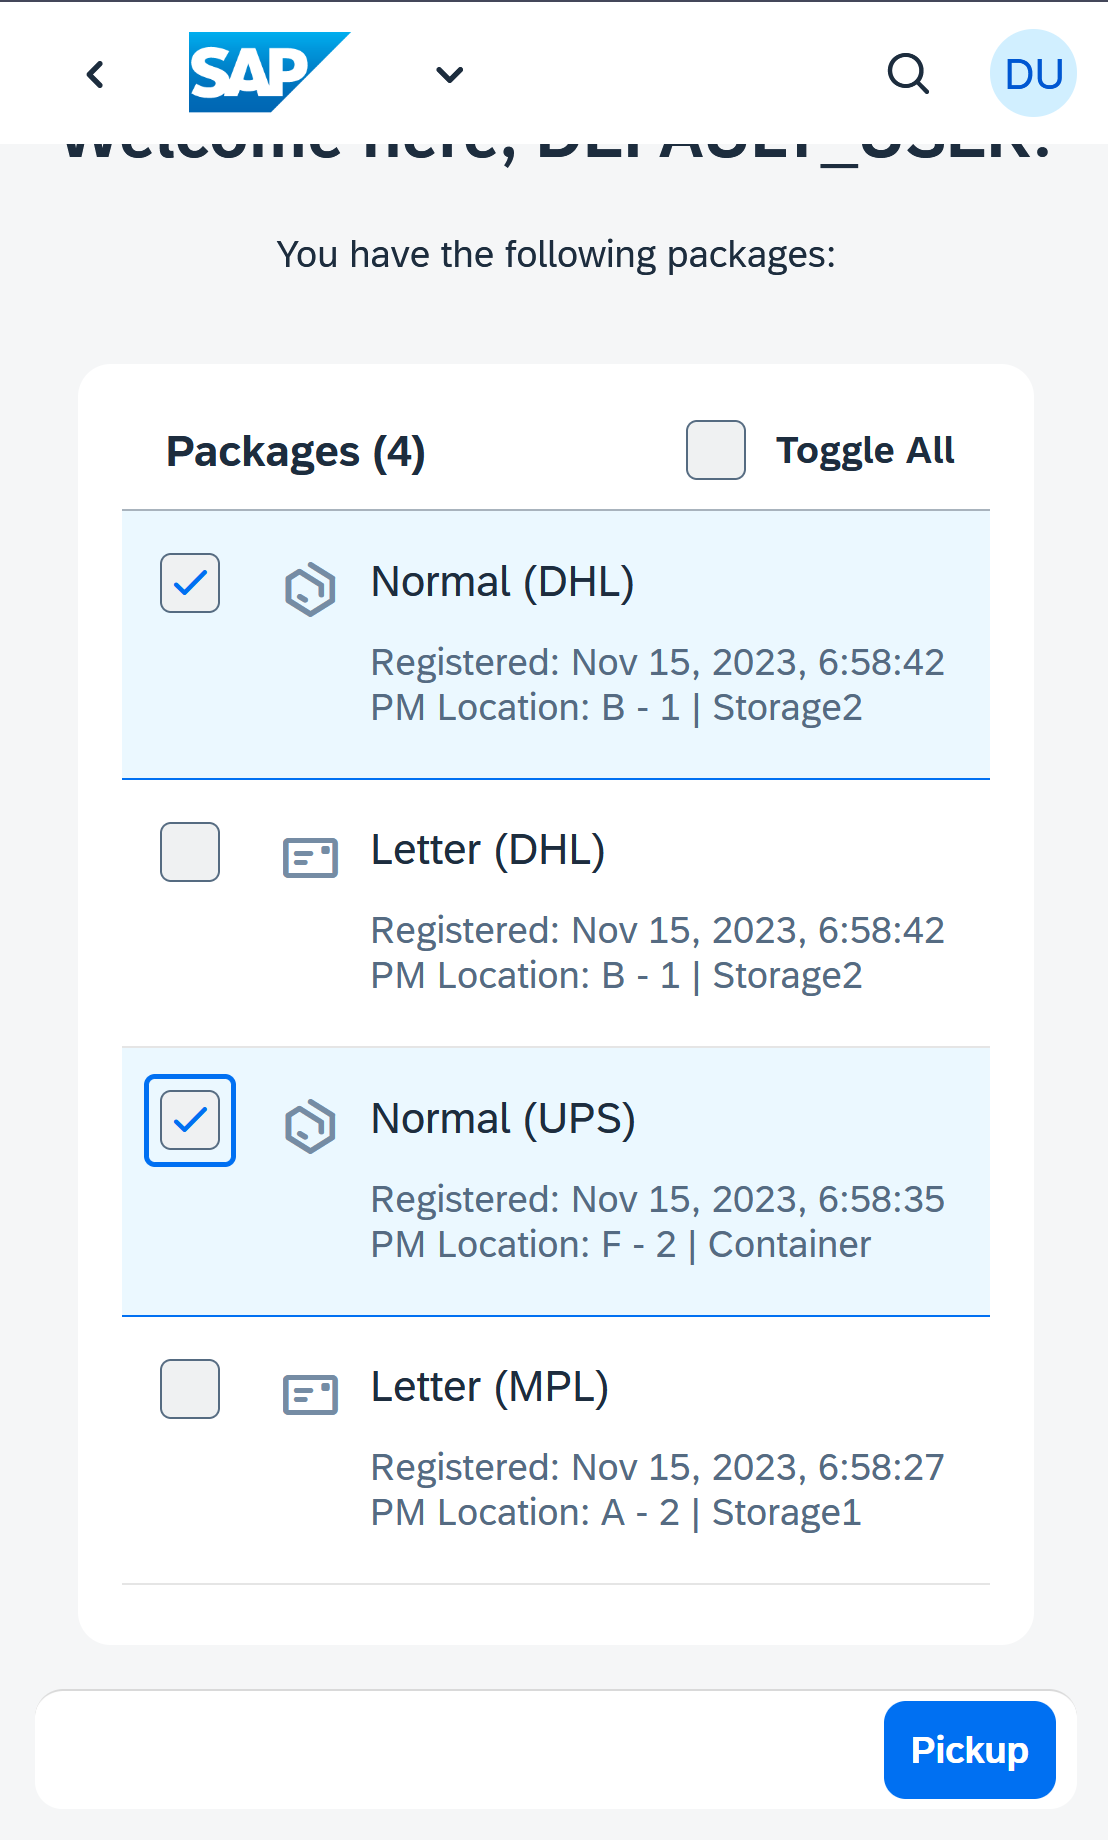
\includegraphics[height=260pt]{images/user_doc/pickup/HomeScreenMultiSelect.png}}
	\caption{Pickup Home Screen - Selection Guide}
	\label{fig:PickupHomeScreen-2}
\end{figure}

\begin{figure}[H]
	\centering
	\subcaptionbox{Home Screen Select All}{
		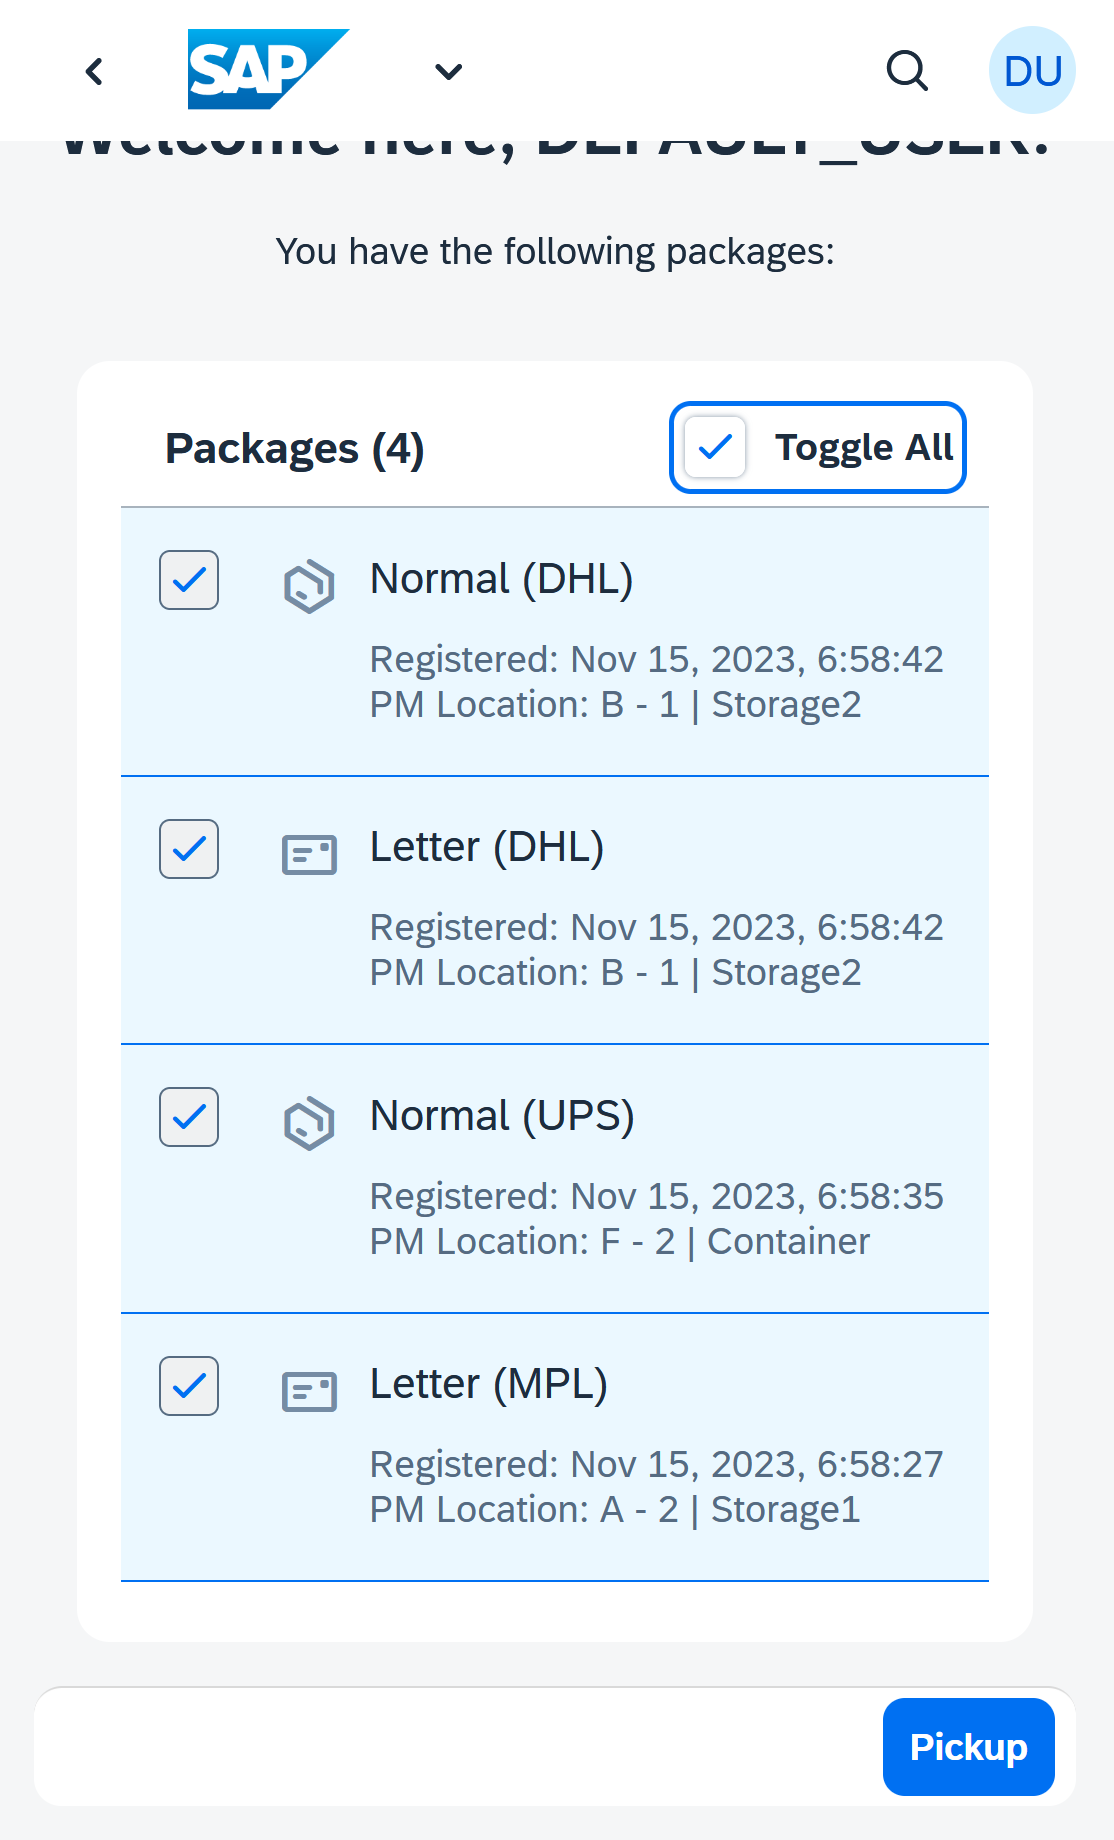
\includegraphics[height=260pt]{images/user_doc/pickup/HomeScreenToggleAll.png}}
	\hspace{5pt}
	\subcaptionbox{Home Screen Deselect All}{
		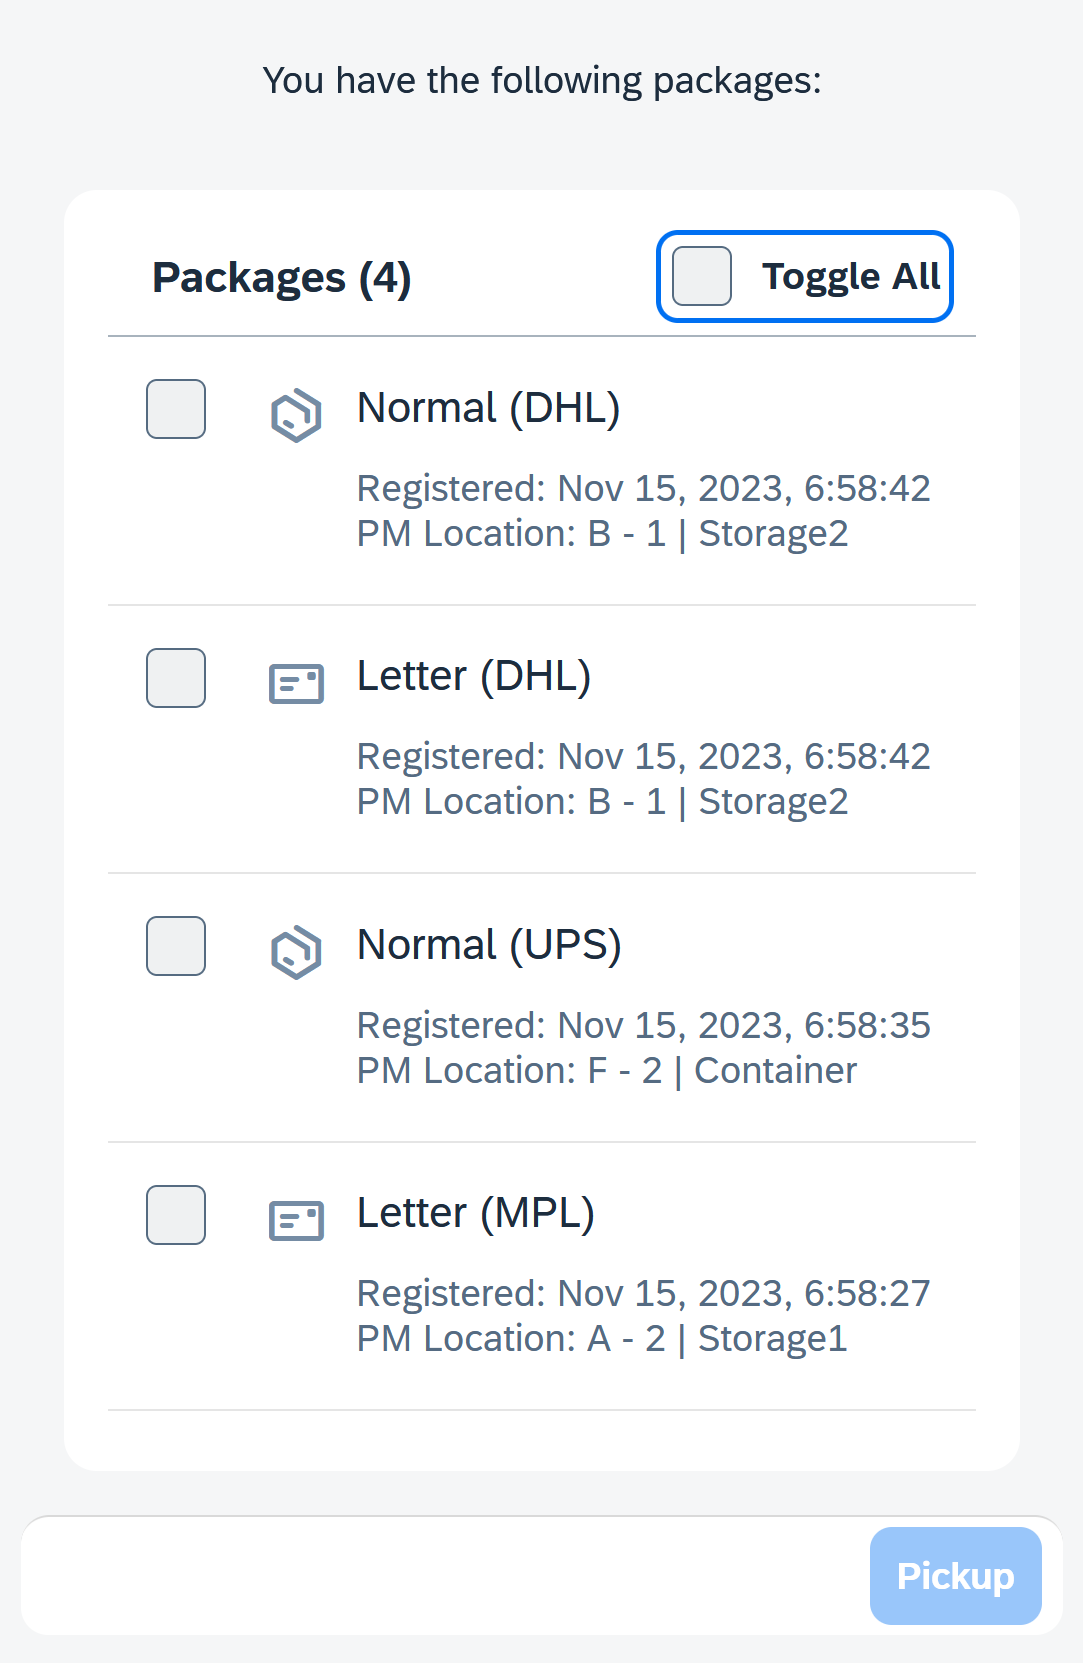
\includegraphics[height=260pt]{images/user_doc/pickup/HomeScreenDeToggleAll.png}}
	\caption{Pickup Home Screen - Selection Guide}
	\label{fig:PickupHomeScreen-2}
\end{figure}

\subsubsection{Home Screen - Pickup}
The "Pickup" button at right bottom corner will only be enabled if at least one package is selected. In case it is enabled, one can pick up the selected packages by left clicking the "Pickup" button, which will trigger a confirmation dialog. If one choose "Cancel", the dialog closes and no modification is made. If one choose "OK", then all packages selected will be marked as pickup, removed from the list and the user will be navigated to the "Done Screen". At this point, the process of the picked up package will be closed, the package data will never be deleted and \textbf{End User} can always go to \textbf{My Packages} application to check the package history.

\begin{figure}[H]
	\centering
	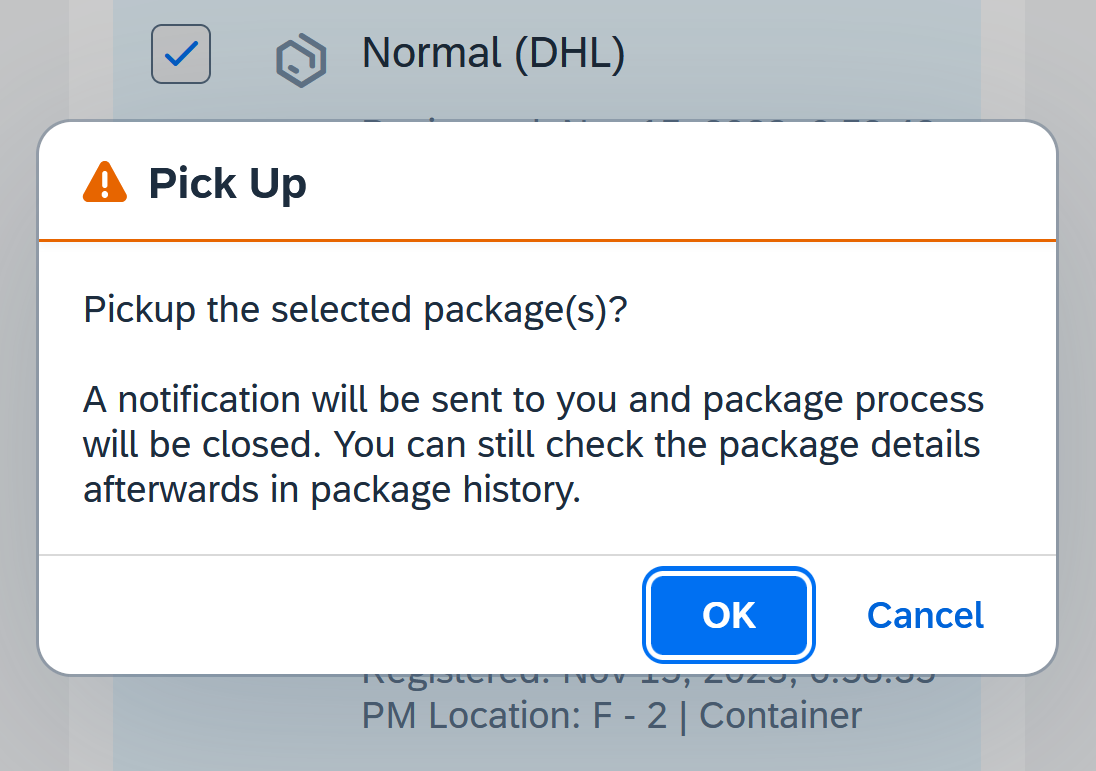
\includegraphics[height=200pt]{images/user_doc/pickup/PickupDialog.png}
	\caption{Pickup Home Screen - Pickup Dialog}
	\label{fig:PickupDialog}
\end{figure}

\subsubsection{Done Screen}

At the "Done Screen", if the \textbf{End User} still have packages to pickup, it will display the list of packages showing their \textbf{type with icon}, \textbf{delivery company} and \textbf{location info}. Otherwise, it displays no more packages. 
User can always navigate back to "Home Screen" by left clicking the "Close" button at the right bottom corner of the page.
From there, a new pickup iteration starts.

\begin{figure}[H]
	\centering
	\subcaptionbox{Done Screen with Packages}{
		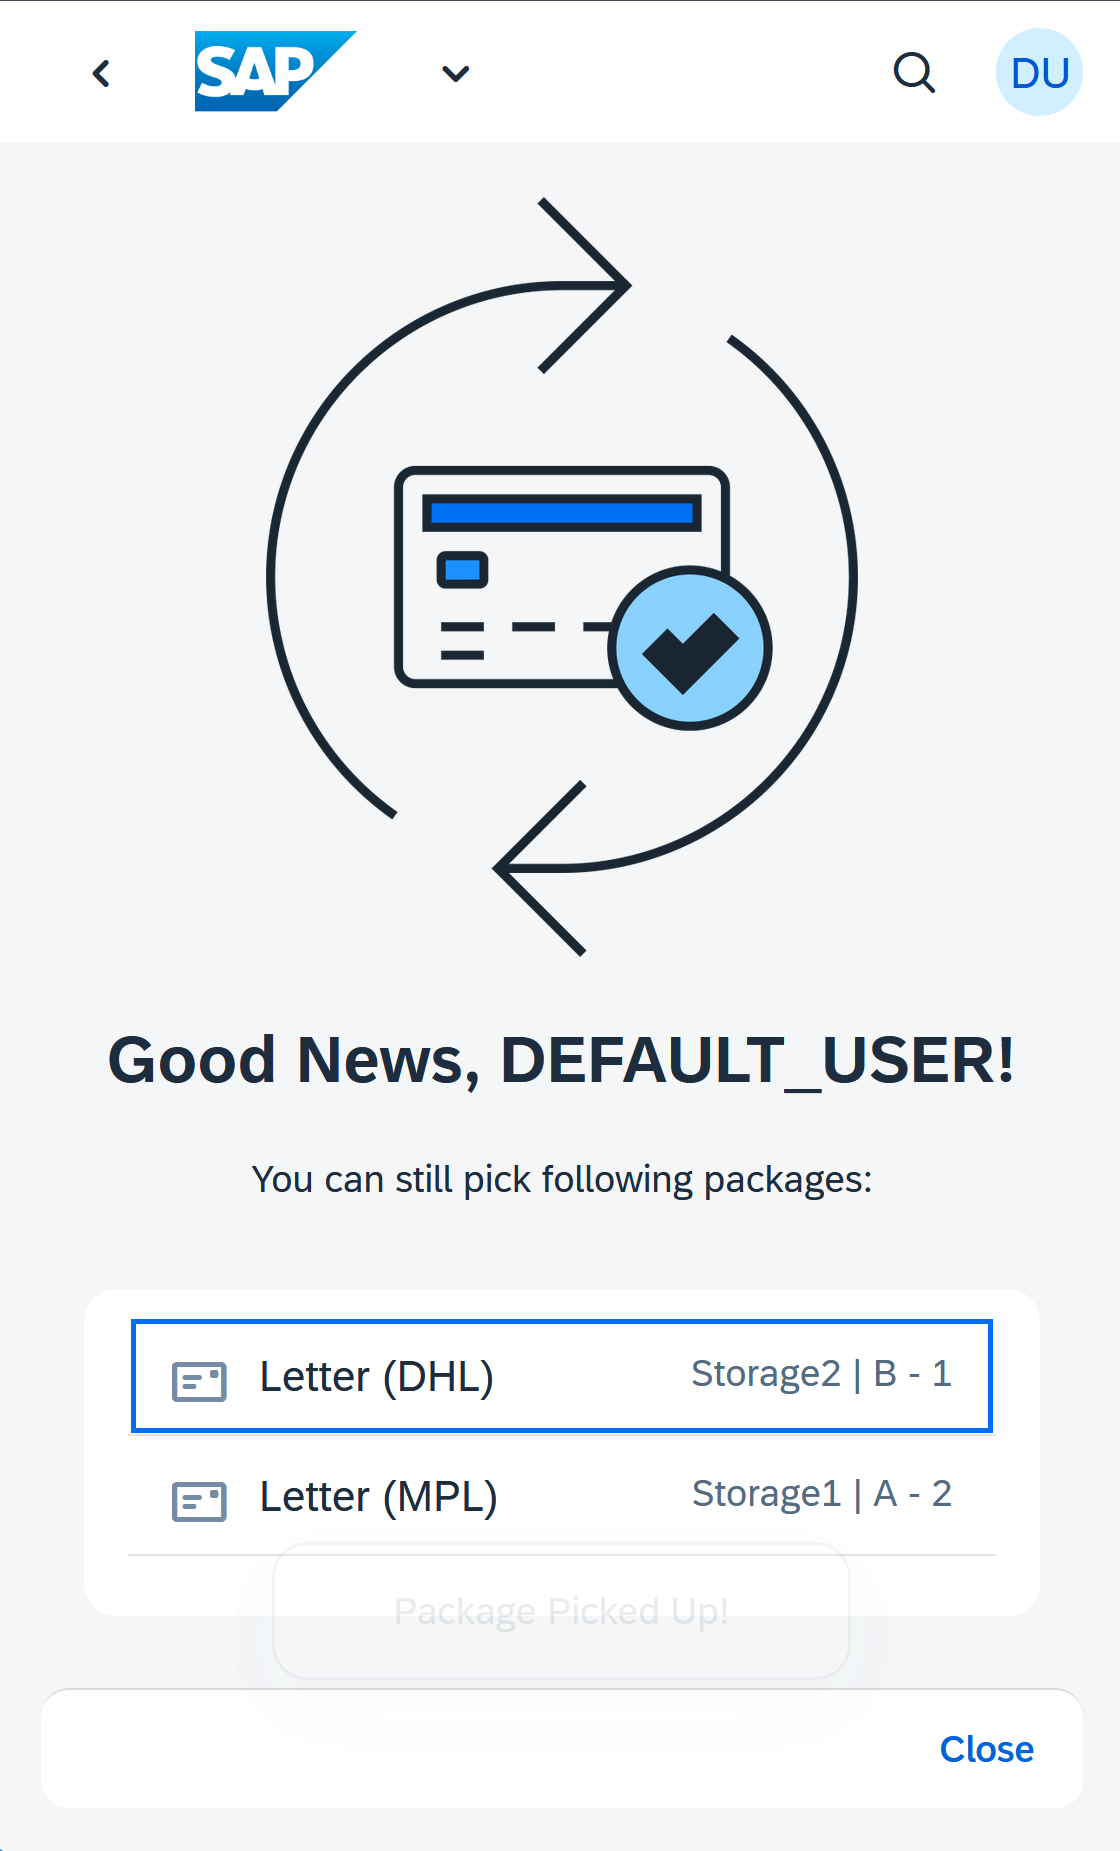
\includegraphics[width=0.45\linewidth]{images/user_doc/pickup/DoneScreenRemainPackages.png}}
	\hspace{5pt}
	\subcaptionbox{Done Screen without Packages}{
		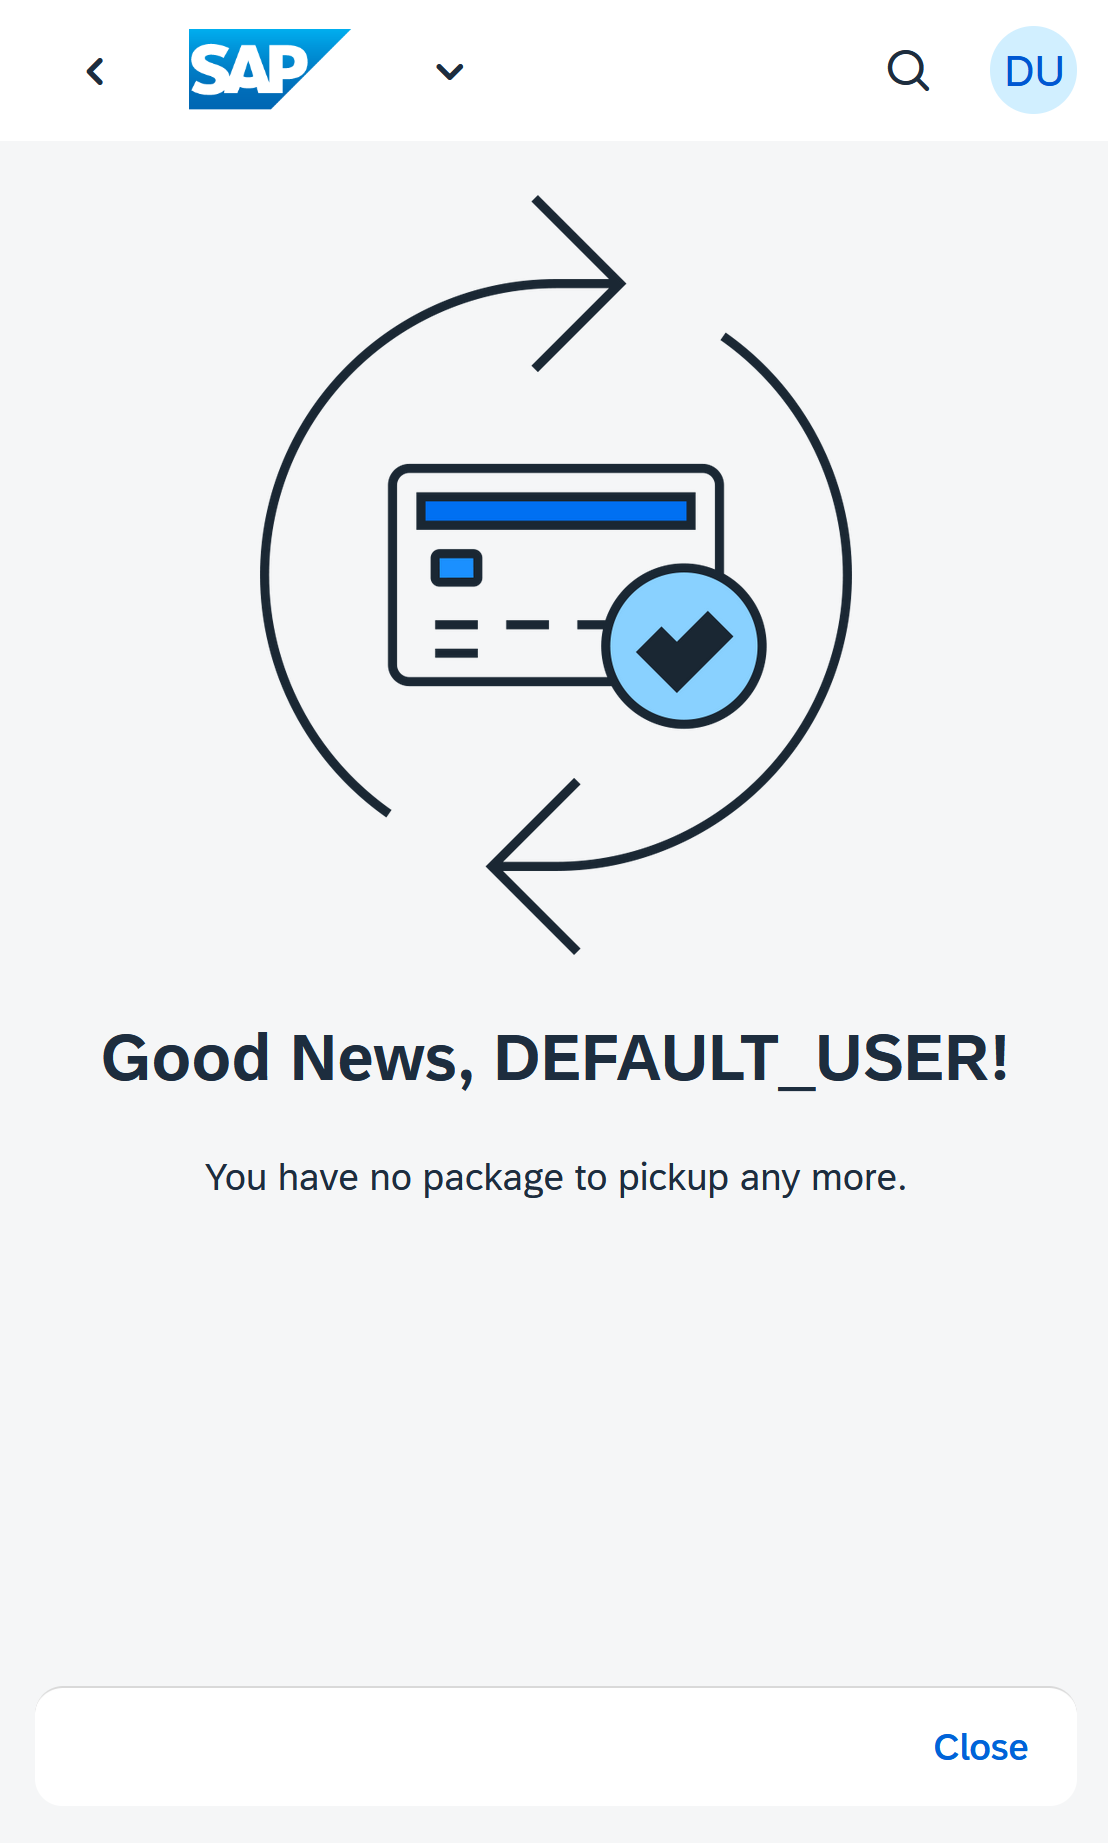
\includegraphics[width=0.45\linewidth]{images/user_doc/pickup/DoneScreenNoPackage.png}}
	\caption{Pickup Done Screen - Package Existence Guide}
	\label{fig:PickupHomeScreen-1}
\end{figure}

\pagebreak

\section{Receptionist}

As a logged in \textbf{Receptionist}, one is granted to access the two applications under the \textbf{Parcel Handling} section, namely \textbf{Register Packages} and \textbf{Manage Packages}. One can quick jump to the section by left clicking the "Parcel Handling" tab. One can enter the application by left click the tiles.

\begin{figure}[H]
	\centering
	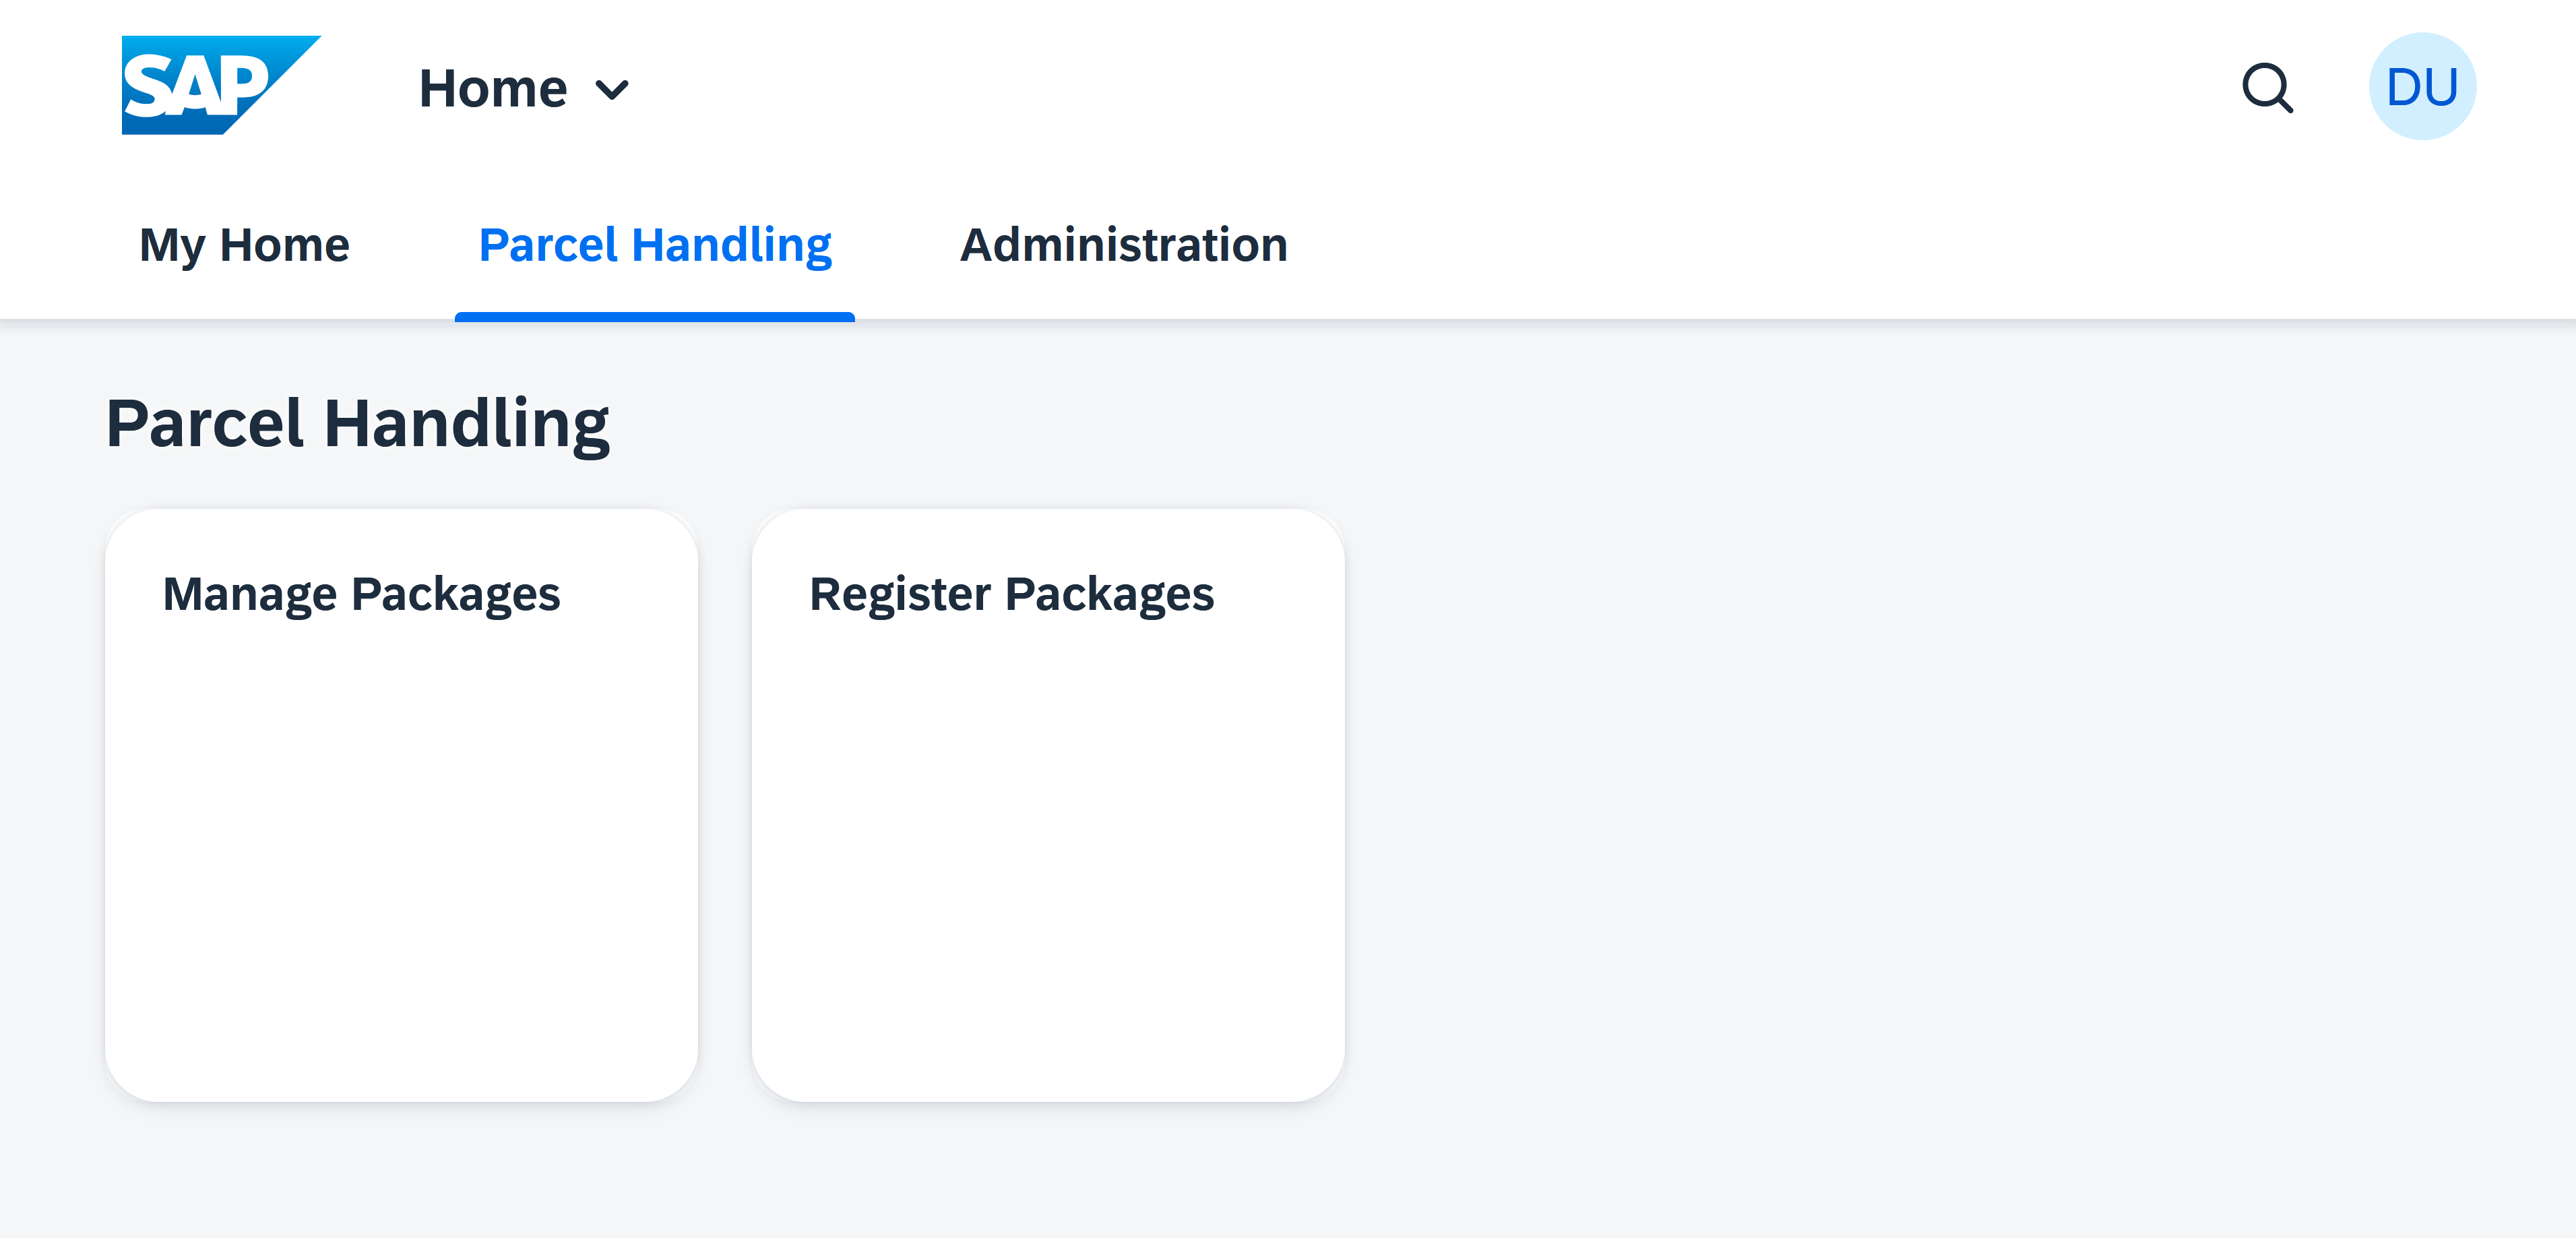
\includegraphics[width=1\linewidth]{images/user_doc/overviews/ParcelHandlingTab.png}
	\caption{Parcel Handling Applications}
	\label{fig:PHApplications}
\end{figure}


\subsection{Register Packages}
\subsubsection{User Stories}
\subsubsection{User Diagram}
\subsubsection{UX Guide}

\subsection{Manage Packages}                     

\pagebreak

\section{Facility Manager}

As a logged in \textbf{Facility Manager}, one is granted to access the two applications under the \textbf{Administration} section, namely \textbf{Manage Companies} and \textbf{Manage Storage}. One can quick jump to the section by left clicking the "Administration" tab. One can enter the application by left click the tiles.

\begin{figure}[H]
	\centering
	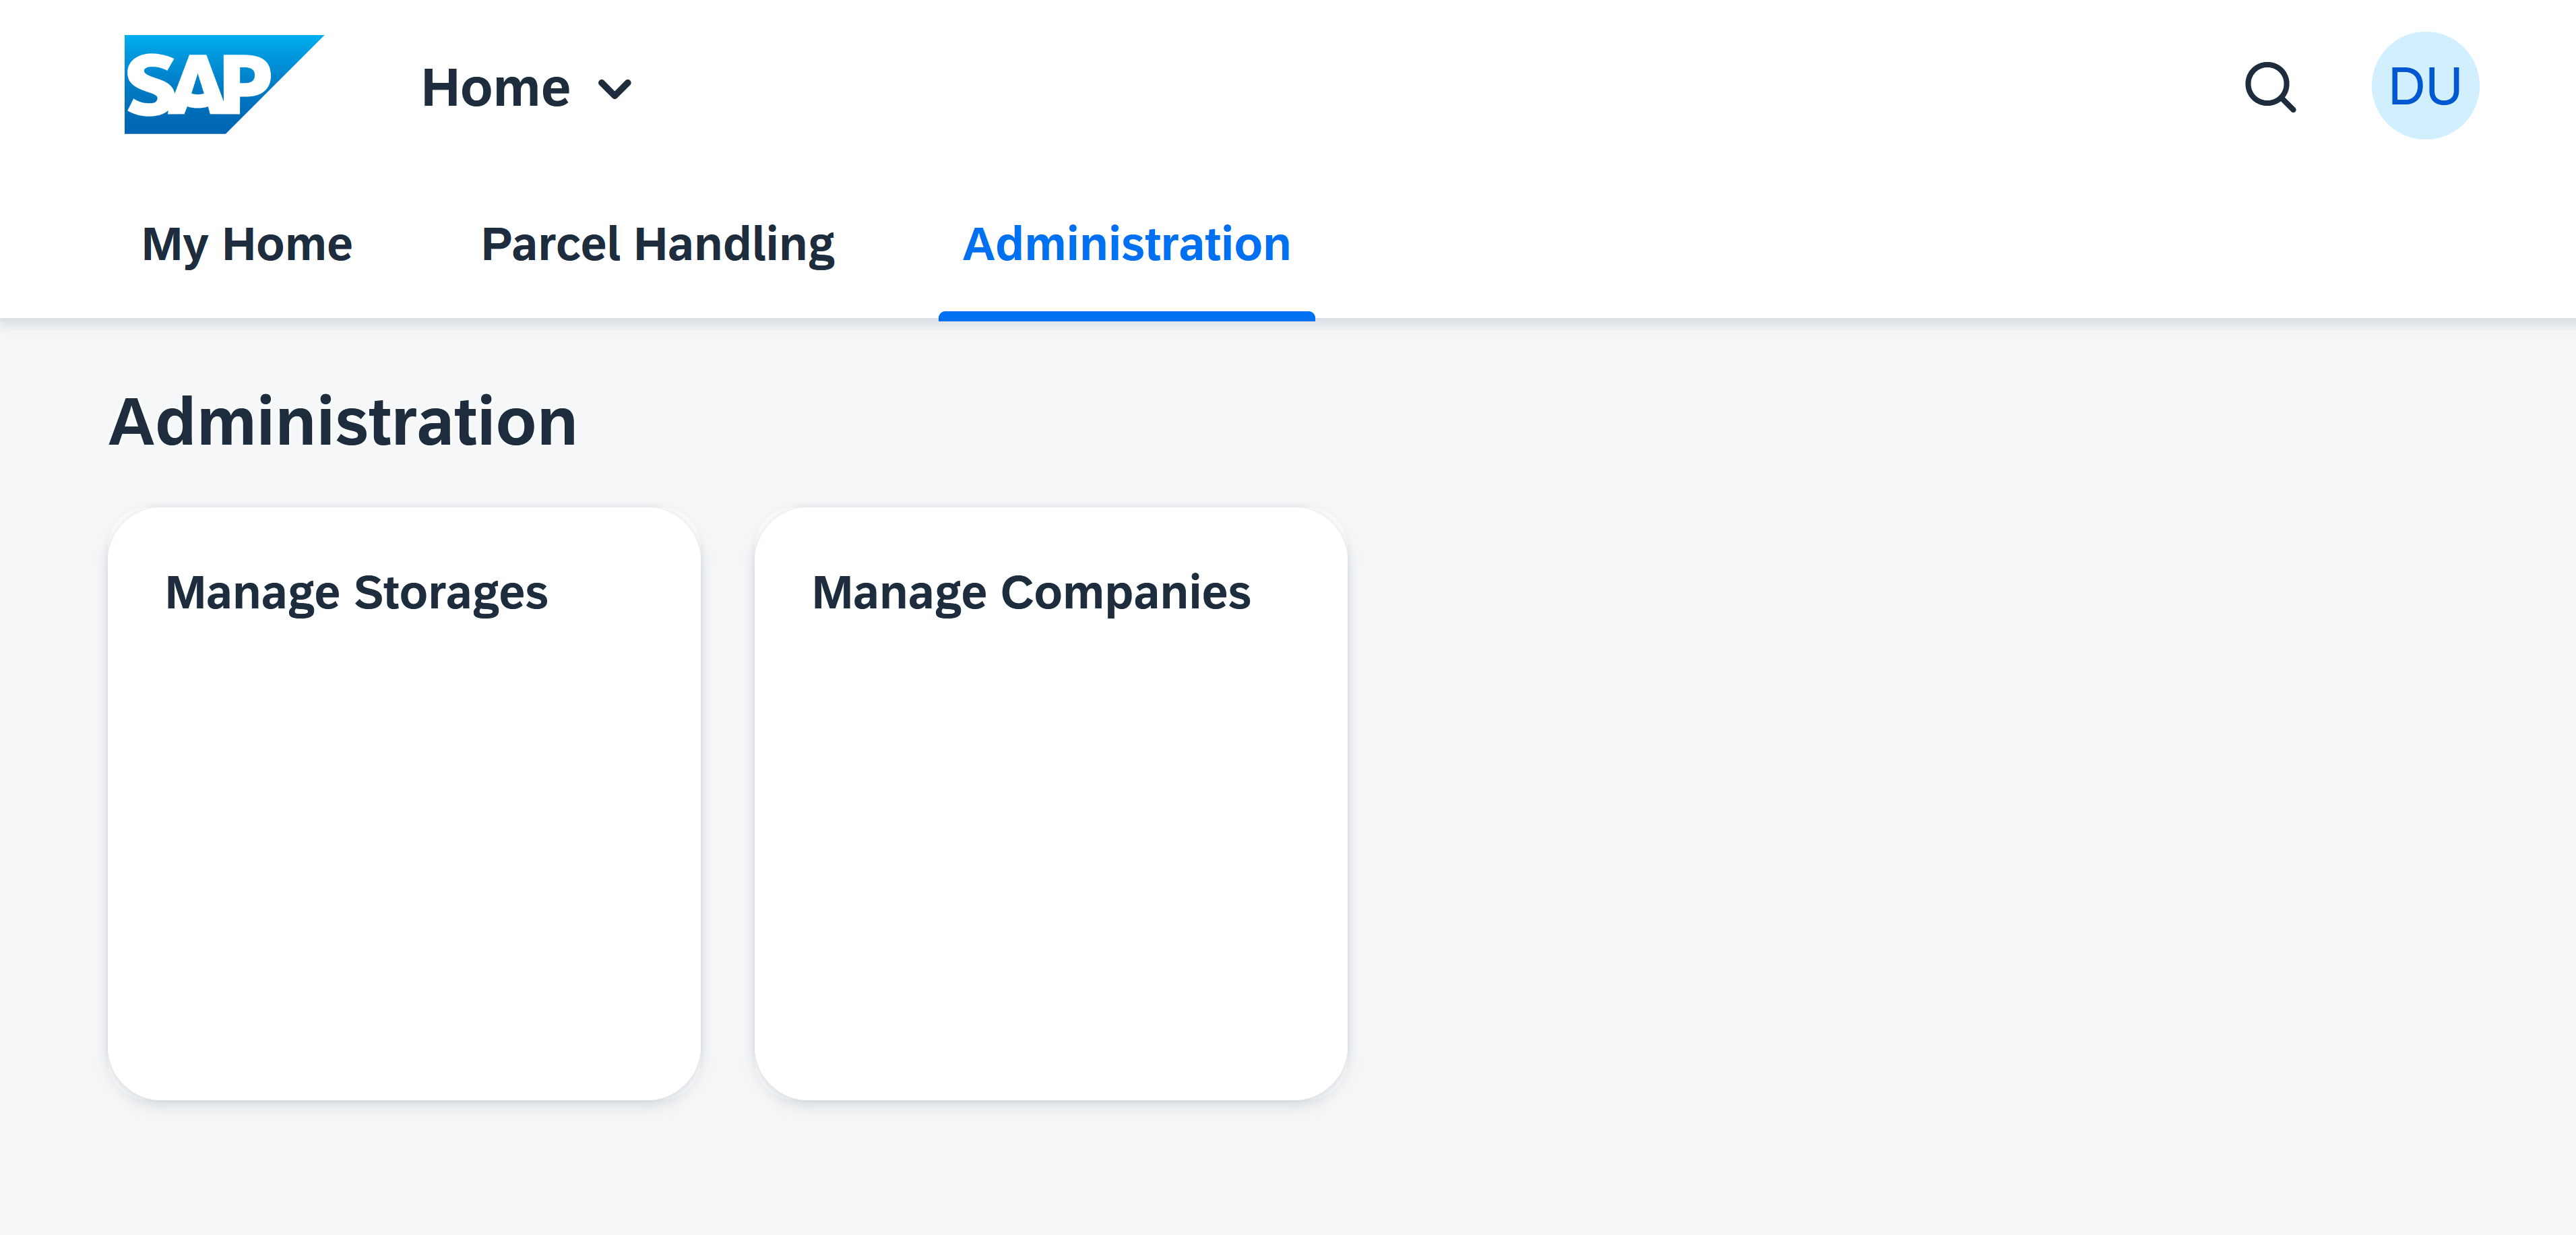
\includegraphics[width=1\linewidth]{images/user_doc/overviews/AdminTab.png}
	\caption{Administration Applications}
	\label{fig:AdministrationApplications}
\end{figure}


\subsection{Manage Companies}


\subsection{Manage Storage}


\section{Administrator}
As a logged in \textbf{Administrator}, one has access to all the 6 applications. One shall move backward to dedicated sections depends on the needs. 